\documentclass[journal]{IEEEtai}

% ---------------------------------------------------------------------------
% Informe final - Competencia Kaggle tweet-age-2026-puj
% Curso de Procesamiento de Lenguaje Natural - Maestria en IA, PUJ
% ---------------------------------------------------------------------------

\usepackage[utf8]{inputenc}
\usepackage[T1]{fontenc}
\usepackage[spanish,es-tabla]{babel}
\usepackage{graphicx}
\usepackage{float}
\usepackage{caption}
\usepackage{subcaption}
\usepackage{amsmath,amsthm,amssymb}
\usepackage{tabularx}
\usepackage{booktabs}
\usepackage{multirow}
\usepackage{multicol}
\usepackage{hyperref}
\hypersetup{hidelinks}

\AtBeginDocument{%
  \renewcommand{\abstractname}{Resumen}%
  \renewcommand{\tablename}{Tabla}%
  \renewcommand{\figurename}{Figura}%
  \renewcommand{\IEEEkeywordsname}{Palabras clave}%
  \renewcommand{\IEEEImpStatementname}{Declaraci\'on de impacto}%
}

\begin{document}

\title{Predicci\'on de rangos etarios a partir de tweets en espa\~nol mediante t\'ecnicas de procesamiento del lenguaje natural y aprendizaje autom\'atico supervisado}

\author{E.~V.~Rivera~Jim\'enez, J.~G.~Carrillo~Meneses, C.~A.~Garnica~Salazar, y O.~A.~Prieto~Moreno%
\thanks{Los cuatro autores est\'an vinculados a la Maestr\'ia en Inteligencia Artificial, Pontificia Universidad Javeriana, Bogot\'a, Colombia. Correos: riveraev@javeriana.edu.co, carrillojuliang@javeriana.edu.co, carlos\_garnicas@javeriana.edu.co y o-prieto@javeriana.edu.co.}}

\markboth{Journal of IEEE Transactions on Artificial Intelligence, Vol. 00, No. 0, Octubre 2026}{E. Rivera et al.: Predicci\'on de rangos etarios en tweets en espa\~nol}

\maketitle

\begin{abstract}
Este art\'iculo responde una pregunta concreta: hasta d\'onde puede llegar un sistema de PLN cl\'asico ---sin \textit{transformers}, sin \textit{embeddings} y sin LLM--- en la clasificaci\'on del rango de edad de tweets en espa\~nol, y d\'onde est\'a el l\'imite real del dato. Sobre la competencia \texttt{tweet-age-2026-puj} (169.336 tweets de entrenamiento y 112.892 de test, seis rangos de edad y macro-F1 como m\'etrica), se construy\'o una cadena \'integramente cl\'asica de TF-IDF, n-gramas de car\'acter, features artesanales y redes tabulares con p\'erdidas ordinales, validada con cinco particiones agrupadas por cl\'usteres de \textit{near-duplicados} y con reglas de decisi\'on calibradas por clase. El resultado principal es un consenso geom\'etrico de expertos (producto de expertos en espacio logar\'itmico) que alcanz\'o 0.63724 de macro-F1 en el \textit{leaderboard} p\'ublico, superando el baseline inicial (0.55235) en +0.08489, junto con una mejor validaci\'on local de 0.6189929 obtenida por un consenso de nueve modelos y estad\'isticamente significativo frente al campe\'on (5/5 folds, $p = 0.0010$). Una auditor\'ia matem\'atica del s\'implejo de pesos confirm\'o que la soluci\'on habita un \'optimo estacionario ---superficie c\'oncava con v\'ertice en el producto de expertos y calibraci\'on mon\'otona decil a decil--- y el techo del dato qued\'o medido y declarado: 0.642 en el \textit{leaderboard}, con 0.70 fuera de alcance bajo las restricciones vigentes. La b\'usqueda sistem\'atica de se\~nal (220 experimentos registrados) delimit\'o qu\'e t\'ecnicas aportan y cu\'ales no, con falsaciones reproducibles. El trabajo deja tres pr\'acticas transferibles: la validaci\'on agrupada por \textit{near-duplicados} es indispensable, la ordinalidad del problema es explotable y el techo observado pertenece al dato, no al modelo.
\end{abstract}

\begin{IEEEkeywords}
Procesamiento de lenguaje natural, perfilado de autor, clasificaci\'on de texto, m\'etricas macro-F1, validaci\'on cruzada agrupada, ensambles, productos de expertos, reproducibilidad.
\end{IEEEkeywords}

\begin{IEEEImpStatement}
El sistema presentado alcanza 0.63724 de macro-F1 en una competencia real de Kaggle sin usar \textit{transformers}, \textit{embeddings} ni modelos de lenguaje: todo el desempe\~no proviene de representaciones estad\'isticas, features artesanales y modelos cl\'asicos. Los resultados muestran que, en corpus cortos y ruidosos, la calidad del protocolo de validaci\'on y de la regla de decisi\'on pesa tanto como la capacidad del modelo, y que el techo observado pertenece al dato. La auditor\'ia matem\'atica del consenso respalda la selecci\'on ante la evaluaci\'on privada y ofrece un criterio replicable para decidir cu\'ando detener la b\'usqueda de se\~nal.
\end{IEEEImpStatement}

% ===========================================================================
\section{Introducci\'on}
% ===========================================================================

\IEEEPARstart{E}{l} perfilado de autor consiste en inferir atributos demogr\'aficos ---edad, g\'enero, procedencia--- a partir de la forma en que una persona escribe. La edad es, de esos atributos, uno de los m\'as dif\'iciles: el vocabulario de dos cohortes vecinas se solapa casi por completo y la se\~nal discriminante vive en detalles estil\'isticos d\'ebiles y distribuidos, como la longitud de las oraciones, el uso de puntuaci\'on o la preferencia l\'exica \cite{nguyen2013,nguyen2014}. Schler et al.\ establecieron en blogs el esquema de seis rangos que hoy es est\'andar ---13-17, 18-24, 25-34, 35-49, 50-64 y 65 en adelante--- y mostraron que la separaci\'on entre cohortes es sistem\'atica pero modesta \cite{schler2006}; Argamon et al.\ profundizaron en las marcas estil\'isticas que la sostienen \cite{argamon2007}, y la serie de laboratorios PAN convirti\'o el problema en una tarea de evaluaci\'on comparable durante siete ediciones \cite{rangel2013,rangel2015,rangel2017,rangel2019}. En Twitter, la tarea es a\'un m\'as dif\'icil que en textos largos: los mensajes son cortos, ruidosos y multiling\"ues, y los estudios espec\'ificos han reportado techos bajos incluso con modelos poderosos \cite{nguyen2011,sap2014,morganlopez2017}.

Este art\'iculo documenta una exploraci\'on completa del problema bajo una restricci\'on deliberada y severa: la competencia \texttt{tweet-age-2026-puj}, organizada en el curso de Procesamiento de Lenguaje Natural de la Maestr\'ia en Inteligencia Artificial de la Pontificia Universidad Javeriana, proh\'ibe usar \textit{transformers}, modelos de lenguaje y, en general, cualquier modelo de vectorizaci\'on o \textit{embedding}, preentrenado o entrenado desde cero. Todo el desempe\~no debe provenir, por tanto, de representaciones estad\'isticas como TF-IDF, de features artesanales y de clasificadores cl\'asicos. El corpus contiene 169.336 tweets de entrenamiento y 112.892 de test, etiquetados en los seis rangos de edad, y la m\'etrica oficial es la macro-F1 sin ponderar.

La pregunta que organiza el trabajo es la siguiente: \emph{\textquestiondown hasta d\'onde puede llegar un sistema de PLN cl\'asico en la clasificaci\'on del rango de edad de tweets en espa\~nol, y d\'onde est\'a el l\'imite real del dato?} La respuesta se articula en cuatro contribuciones.

\begin{enumerate}
\item Un consenso geom\'etrico de expertos cl\'asicos (producto de expertos en espacio logar\'itmico) con una regla de decisi\'on calibrada por clase alcanz\'o \textbf{0.63724 de macro-F1 en el \textit{leaderboard}} (referencia 57283487), una mejora de \textbf{+0.08489} sobre el baseline inicial de 0.55235.
\item La \textbf{mejor validaci\'on local} del proyecto es 0.6189929 de macro-F1 (particiones agrupadas, leave-one-fold-out) con un consenso de nueve modelos, estad\'isticamente significativo frente al campe\'on (5/5 folds positivos, bootstrap pareado $p = 0.0010$).
\item El \textbf{techo del dato} qued\'o medido y declarado: 0.642 de macro-F1 en el \textit{leaderboard} como m\'aximo alcanzable, con el objetivo de 0.70 refutado por argumentos de informaci\'on disponible.
\item Una \textbf{b\'usqueda sistem\'atica de se\~nal} (220 experimentos registrados) delimit\'o qu\'e t\'ecnicas aportan y cu\'ales no, con falsaciones reproducibles que incluyen distancias ordinales alternativas, transformaciones de la matriz de features, arquitecturas de atenci\'on y familias completas de operadores de consenso.
\end{enumerate}

El resto del art\'iculo se organiza as\'i. La Secci\'on~II revisa los trabajos relacionados en cuatro corrientes y precisa qu\'e se tom\'o de cada una. La Secci\'on~III describe el corpus y los hallazgos del an\'alisis exploratorio, con \'enfasis en el riesgo de \textit{near-duplicados}. La Secci\'on~IV fija el protocolo de validaci\'on y las decisiones fundacionales que condicionaron todo lo dem\'as. La Secci\'on~V presenta la representaci\'on, la matriz de features y la l\'inea base. La Secci\'on~VI analiza en detalle el campe\'on: el consenso geom\'etrico de seis expertos. La Secci\'on~VII contrasta lo que funcion\'o con lo que no, mediante falsaciones documentadas. La Secci\'on~VIII describe la frontera 2026 ---la mejor validaci\'on local y la auditor\'ia matem\'atica del consenso--- y la Secci\'on~IX cierra la validaci\'on estad\'istica. Las Secciones~X y XI discuten las limitaciones y responden la pregunta de investigaci\'on.

% ===========================================================================
\section{Trabajos relacionados}
% ===========================================================================

El problema de inferir la edad del autor de un texto se ha abordado desde cuatro corrientes que convergen en este proyecto: el perfilado de autor cl\'asico, las representaciones estad\'isticas de texto, el tratamiento de la ordinalidad y las redes tabulares con ensambles y reglas de decisi\'on.

\subsection{Perfilado de autor y edad}

Schler et al.\ fijaron el esquema de seis rangos de edad y demostraron, sobre blogs, que las diferencias l\'exicas entre cohortes son medibles pero peque\~nas \cite{schler2006}. Argamon et al.\ caracterizaron esas diferencias como se\~nal estil\'istica m\'as que tem\'atica \cite{argamon2007}. En redes sociales, Nguyen et al.\ mostraron que la predicci\'on de edad en Twitter es notablemente m\'as dif\'icil que en textos largos y que los clasificadores tienden a confundir cohortes adyacentes \cite{nguyen2011,nguyen2013,nguyen2014}; Sap et al.\ encontraron el mismo patr\'on en usuarios de Twitter en ingl\'es \cite{sap2014}, y Morgan-L\'opez et al.\ lo confirmaron en aplicaciones de vigilancia epidemiol\'ogica \cite{morganlopez2017}. Los laboratorios PAN estandarizaron la evaluaci\'on del perfilado de autor y documentaron a\~no tras a\~no techos modestos en la tarea de edad \cite{rangel2013,rangel2014,rangel2015,rangel2016,rangel2017,rangel2018,rangel2019}. Verhoeven et al.\ aportaron evidencia equivalente en neerland\'es \cite{verhoeven2014,verhoeven2016}, Flekova y Gurevych vincularon la edad con rasgos de personalidad en Twitter \cite{flekova2013}, Hovy y Prabhumoye revisaron los sesgos y factores demogr\'aficos que atraviesan el PLN \cite{hovy2018}, y Liu et al.\ mostraron que la se\~nal demogr\'afica es fr\'agil ante cambios de dominio \cite{liu2021}. De esta corriente se tom\'o el esquema de etiquetas, la expectativa de un techo bajo y la hip\'otesis de trabajo central: el error se concentra en las fronteras entre cohortes vecinas.

\subsection{Representaci\'on estad\'istica y NB-SVM}

Wang y Manning mostraron que un clasificador Naive Bayes-SVM sobre n-gramas de palabra y car\'acter es un baseline notablemente competitivo para clasificaci\'on de texto \cite{wang2012}, y Mukherjee y Liu formalizaron el cociente logar\'itmico de cuentas que lo sustenta \cite{mukherjee2010}. Sapkota et al.\ documentaron que los n-gramas de car\'acter capturan informaci\'on estil\'istica valiosa para el perfilado de autor \cite{sapkota2013,sapkota2015}, L\'opez-Monroy et al.\ obtuvieron resultados similares en espa\~nol \cite{lopezmonroy2013} y Monroe et al.\ propusieron el an\'alisis de log-odds con prior Dirichlet, que se us\'o aqu\'i para inspeccionar l\'exico discriminante \cite{monroe2008}. De esta corriente provienen el baseline NB-SVM de la versi\'on~V12 y la apuesta por n-gramas de car\'acter, que result\'o ser la representaci\'on dominante del proyecto.

\subsection{Ordinalidad y distancias entre distribuciones}

Frank y Hall formalizaron la clasificaci\'on ordinal mediante cadenas de umbrales \cite{frank2001}, y Cao et al.\ reintrodujeron la idea en redes neuronales con CORAL \cite{cao2020}; D\'iaz y Marathe propusieron etiquetas suaves ordinales para preservar la estructura de vecindad entre clases \cite{diaz2019}. En paralelo, la distancia de Cram\'er--von Mises \cite{cramer1928,vonmises1931}, la estad\'istica de energ\'ia de Sz\'ekely y Rizzo \cite{szekely2013} y la p\'erdida de Wasserstein de Frogner et al.\ \cite{frogner2015} ofrecen maneras de penalizar distancias entre distribuciones acumuladas, que es justamente lo que el problema requiere: castigar m\'as una confusi\'on lejana que una adyacente. De esta corriente se adopt\'o la p\'erdida de Cram\'er $L_2$ sobre la CDF y la cadena de umbrales; el cap\'itulo de falsaciones de la Secci\'on~VII documenta qu\'e variantes de la familia no funcionaron.

\subsection{Redes tabulares, ensambles y decisi\'on}

Gorishniy et al.\ revisaron sistem\'aticamente el aprendizaje profundo sobre datos tabulares y mostraron que las redes residuales con compuertas de atenci\'on compiten con los \'arboles de gradiente \cite{gorishniy2021}. Las compuertas Squeeze-and-Excitation \cite{hu2018}, las conexiones densas de DenseNet \cite{huang2017}, el promedio de pesos estoc\'astico (SWA) \cite{izmailov2018}, el enfriamiento cosenoidal \cite{loshchilov2017}, el suavizado de etiquetas \cite{szegedy2016,muller2019} y las redes autonormalizantes \cite{klambauer2017} aportaron las piezas de arquitectura y regularizaci\'on. Para combinar modelos se usaron el producto de expertos de Hinton \cite{hinton2002} y los \textit{pools} logar\'itmicos de Heskes \cite{heskes1998}, sobre miembros de boosting como LightGBM \cite{ke2017} y CatBoost \cite{prokhorenkova2018}. La decisi\'on final se apoya en la teor\'ia de umbralizaci\'on \'optima de F-medidas: Lipton et al.\ derivaron la regla de multiplicadores por clase que se us\'o como regla \textit{plug-in} \cite{lipton2014}, y los trabajos de Parambath et al., Waegeman et al., Narasimhan et al.\ y Eban et al.\ cubren el problema de optimizar F-medidas directamente \cite{parambath2014,waegeman2014,narasimhan2015,eban2017}.

\subsection{Fugas de informaci\'on y paradojas de agregaci\'on}

Kaufman et al.\ sistematizaron el problema de las fugas de datos en miner\'ia de datos y advirtieron que los duplicados entre particiones inflan las m\'etricas de forma silenciosa \cite{kaufman2012}; ese diagn\'ostico guio el protocolo de validaci\'on de la Secci\'on~IV. Por \'ultimo, la paradoja de Simpson \cite{simpson1951} explica por qu\'e las reglas de decisi\'on desacopladas por segmento, que mejoran una m\'etrica local, pueden degradar la macro-F1 global: los falsos positivos y falsos negativos de los segmentos se suman en el mismo denominador.

A diferencia de la mayor parte de la literatura reciente de edad y perfilado, que explota \textit{embeddings} y \textit{transformers}, este trabajo mide con precisi\'on qu\'e se puede lograr cuando esas herramientas est\'an prohibidas, y aporta como contribuci\'on metodol\'ogica la combinaci\'on de validaci\'on agrupada por \textit{near-duplicados}, consenso multiplicativo y regla de decisi\'on calibrada, con un techo declarado y verificado.

% ===========================================================================
\section{Datos y an\'alisis exploratorio}
% ===========================================================================

El corpus de la competencia est\'a compuesto por tres archivos con estructura id\'entica a la de una tarea supervisada convencional: un conjunto de entrenamiento etiquetado, un conjunto de test sin etiqueta y una plantilla de env\'io. La Tabla~\ref{tab:datos} resume sus dimensiones y la Tabla~\ref{tab:propiedades} las propiedades del texto que condicionaron todas las decisiones posteriores.

\begin{table}[htbp]
\centering
\caption{Archivos del corpus de la competencia.}
\label{tab:datos}
\footnotesize
\setlength{\tabcolsep}{4pt}
\begin{tabular}{lccc}
\toprule
Archivo & Filas & Columnas & Separador \\
\midrule
\texttt{age\_train.csv} & 169.336 & \texttt{id;text;age\_range} & ; \\
\texttt{age\_test.csv} & 112.892 & \texttt{id;text} & ; \\
\texttt{age\_submission.csv} & 112.892 & \texttt{id,age\_range} & , \\
\bottomrule
\end{tabular}
\end{table}

\begin{table}[htbp]
\centering
\caption{Propiedades verificadas del corpus y su tratamiento.}
\label{tab:propiedades}
\begin{tabular}{p{0.52\columnwidth}p{0.40\columnwidth}}
\toprule
Propiedad & Tratamiento \\
\midrule
Clases casi balanceadas por dise\~no: 17.0\%, 16.9\%, 16.7\%, 16.7\%, 16.6\% y 16.0\% & Nada que corregir; macro-F1 como m\'etrica \\
Ancho fijo de 140 caracteres con relleno de espacios (mediana real de 93) & Recorte del relleno en la carga (Decisi\'on 2) \\
Alfabeto transliterado a ASCII: \'unico car\'acter no ASCII (\textquestiondown, 88 apariciones) & Features de emoji descartadas (Decisi\'on 3) \\
104 textos vac\'ios en train y 62 en test & Se conservan; los modelos los resuelven con el prior \\
643 filas (0.38\%) con etiquetas contradictorias para el mismo texto & Ruido irreducible; se documenta \\
\texttt{id} sin capacidad predictiva (desviaci\'on m\'axima de 1.25\,pp entre deciles) & Descartado como feature \\
Sin metadatos: no hay usuario, fecha, biograf\'ia ni seguidores & Toda la se\~nal es textual \\
\bottomrule
\end{tabular}
\end{table}

\subsection{Balance de clases y artefactos del corpus}

Las seis clases est\'an casi balanceadas por construcci\'on: 13-17 concentra el 17.0\% de las filas, 18-24 el 16.9\%, 25-34 y 35-49 el 16.7\% cada una, 50-64 el 16.6\% y 65-xx el 16.0\%. El balance descarta el desbalanceo como explicaci\'on de los errores y permite leer la macro-F1 como un promedio honesto de seis problemas de dificultad comparable. La Fig.~\ref{fig:clases} muestra esa distribuci\'on junto con las longitudes: los tweets fueron almacenados en ancho fijo de 140 caracteres con relleno de espacios ---artefacto de exportaci\'on, no se\~nal, que se elimina en la carga--- y la mediana real tras el recorte es de 93 caracteres, con una distribuci\'on de palabras que se concentra entre 5 y 25.

\begin{figure}[htbp]
\centering
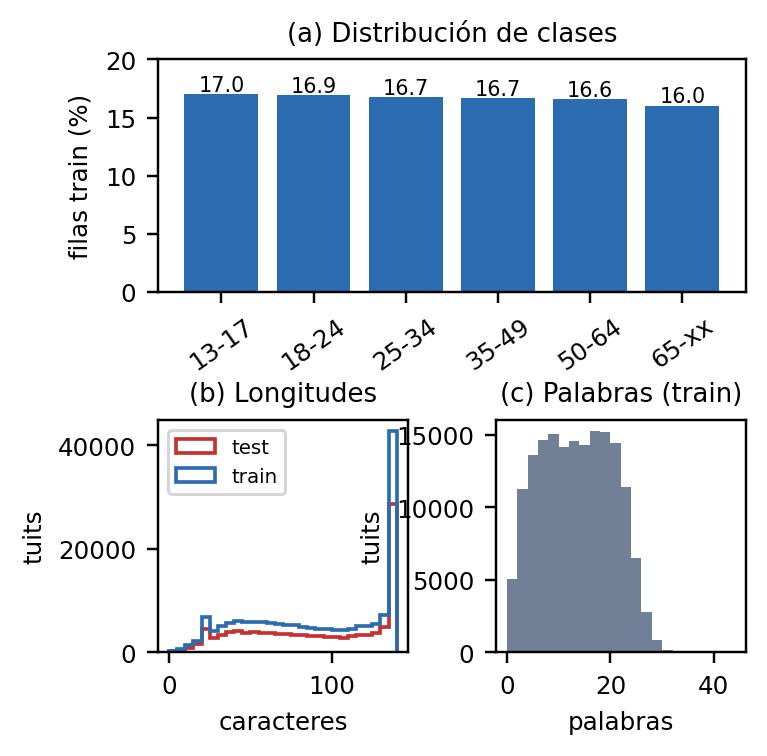
\includegraphics[width=\columnwidth]{figuras/fig_01_eda.png}
\caption{Distribuci\'on de clases y longitudes del corpus. Las seis cohortes est\'an casi balanceadas por dise\~no; las longitudes en caracteres de train y test son indistinguibles, sin se\~nal de cambio de dominio entre particiones.}
\label{fig:clases}
\end{figure}

Un segundo artefacto es la transliteraci\'on del corpus a ASCII: el alfabeto completo tiene 96 caracteres y el \'unico no ASCII es el signo de apertura de interrogaci\'on, con 88 apariciones. No hay tildes, ni e\~ne, ni emojis, ni puntuaci\'on tipogr\'afica. Esa p\'erdida es una limitaci\'on declarada del dato, pero tiene una consecuencia metodol\'ogica \'util: las features de emoji no tienen varianza y se descartan, lo que refuerza la apuesta por los n-gramas de car\'acter como representaci\'on principal. El corpus tampoco incluye metadatos: no hay identificador de usuario, fecha, biograf\'ia ni contadores sociales, de modo que no es posible agrupar por autor ni explotar se\~nal temporal, y toda la predicci\'on depende del texto. Por decisi\'on expl\'icita del equipo, tampoco se usaron datos externos etiquetados aunque las reglas no los prohibieran, para que la ventaja competitiva fuera atribuible al modelado y no a recursos ajenos al problema.

El an\'alisis l\'exico por clase (Fig.~\ref{fig:terminos}) muestra el patr\'on esperado de vocabulario compartido: los t\'erminos m\'as frecuentes de cada rango son casi los mismos en todos ---\emph{para}, \emph{como}, \emph{esta}, \emph{pero}--- y las diferencias aparecen en los m\'argenes de la lista, con marcas de registro como \emph{quiero} en las cohortes j\'ovenes o referencias institucionales en las mayores. Esta fotograf\'ia anticipa el hallazgo central del an\'alisis de error: la se\~nal discriminante es d\'ebil y estil\'istica, no tem\'atica.

\begin{figure*}[htbp]
\centering
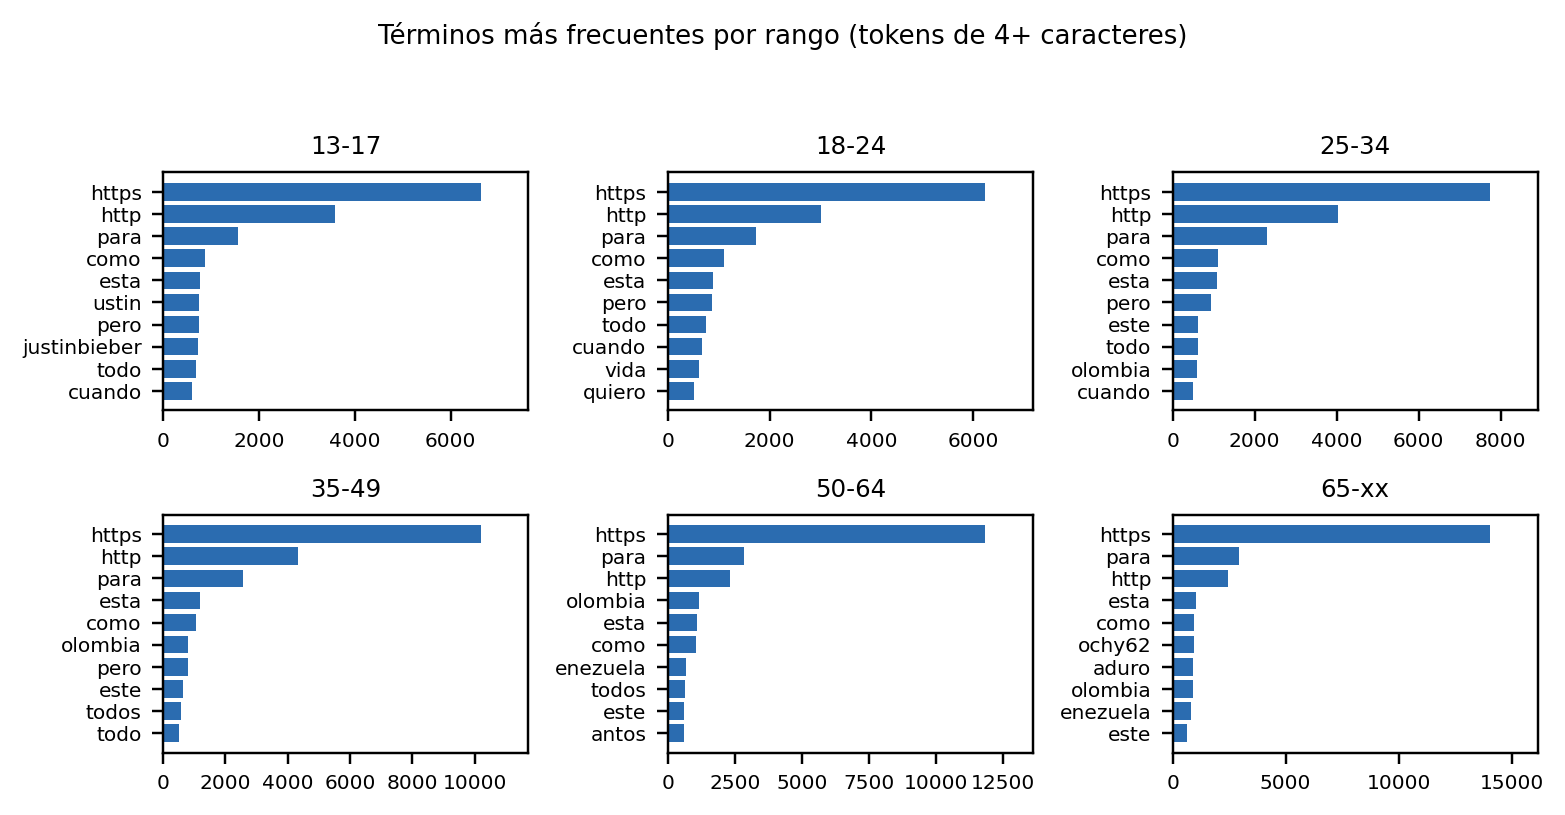
\includegraphics[width=0.98\textwidth]{figuras/fig_02_terminos.png}
\caption{T\'erminos m\'as frecuentes por rango de edad (tokens de cuatro o m\'as caracteres). El n\'ucleo del vocabulario es com\'un a las seis cohortes y las diferencias se concentran en los m\'argenes de cada lista.}
\label{fig:terminos}
\end{figure*}

\subsection{Duplicados y \textit{near-duplicados}: el riesgo dominante}

El hallazgo m\'as importante del an\'alisis exploratorio fue la presencia de contenido repetido entre particiones. El 1.21\% de las filas de test aparece literalmente en train, y un 4.26\% adicional comparte cl\'uster de \textit{near-duplicado} seg\'un una similitud de Jaccard mayor o igual a 0.8 sobre tokens, calculada con \textit{blocking} por tokens raros para hacer viable la comparaci\'on. Sobre el total de 282.228 textos de train y test se identificaron 271.539 cl\'usteres, y el 92.8\% de ellos es de etiqueta \'unica: cuando un texto se repite, casi siempre se repite con la misma etiqueta. La Fig.~\ref{fig:clusters} resume el fen\'omeno.

\begin{figure}[htbp]
\centering
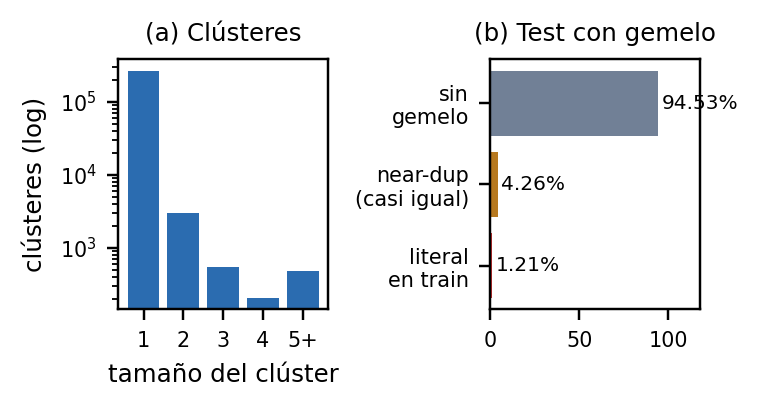
\includegraphics[width=\columnwidth]{figuras/fig_03_clusters.png}
\caption{Tama\~no de los cl\'usteres de \textit{near-duplicados} y proporci\'on del test con gemelo en train. La mayor\'ia de los textos no tiene gemelo (267.287 cl\'usteres unitarios) y, entre los duplicados, dominan los pares (3.012 de 4.252); un 5.5\% del test tiene un gemelo o casi-gemelo etiquetado en train, el riesgo de medici\'on dominante del problema.}
\label{fig:clusters}
\end{figure}

Este fen\'omeno tiene dos lecturas que conviene separar. La primera es competitiva: como el \textit{leaderboard} punt\'ua sobre un test que contiene \textit{near-duplicados} del train, un modelo con capacidad de memorizaci\'on obtiene all\'i una ventaja sistem\'atica. La segunda es metodol\'ogica: si la validaci\'on local reparte al azar textos que son casi id\'enticos, las m\'etricas de desarrollo quedan infladas y las decisiones de modelo se toman sobre una se\~nal falsa. Para cuantificar la magnitud del problema se midi\'o un baseline de memorizaci\'on pura, que consiste en predecir la etiqueta del vecino id\'entico cuando existe: con una partici\'on estratificada ingenua ese baseline alcanza 0.0608 de macro-F1, mientras que con el esquema agrupado que se describe en la Secci\'on~IV cae a 0.0000. La diferencia es la medida exacta del autoenga\~no que habr\'ia contaminado el proyecto.

Para calibrar las escalas se calcularon adem\'as dos suelos de referencia. El azar uniforme sobre seis clases equivale a 0.1667 de macro-F1, y predecir siempre la clase mayoritaria da 0.04854, porque la macro-F1 castiga a las cinco clases que quedan sin recall. Cualquier cifra por encima de 0.5, por tanto, representa se\~nal real, y las diferencias que se reportan en este art\'iculo ---del orden de mil\'esimas--- hay que leerlas en esa escala.

% ===========================================================================
\section{Metodolog\'ia y decisiones fundacionales}
% ===========================================================================

El proyecto fij\'o su protocolo antes de entrenar el primer modelo y lo aplic\'o sin excepciones durante 220 experimentos. La Tabla~\ref{tab:decisiones} resume las decisiones que resultaron cruciales y su impacto; las subsecciones siguientes detallan las dos m\'as costosas de revertir.

\subsection{Marco metodol\'ogico: CRISP-DM}

El proyecto se condujo con \textbf{CRISP-DM} (\textit{Cross-Industry Standard Process for Data
Mining}; Wirth y Hipp, 2000) como metodolog\'ia principal \cite{wirth2000}, aplicada de forma
iterativa sobre sus seis fases. La \textbf{comprensi\'on del negocio} fij\'o la tarea, la m\'etrica
(macro-F1) y las restricciones de la competencia (sin \textit{transformers}, \textit{embeddings}
ni modelos de lenguaje), junto con la disciplina de env\'ios que se describe m\'as abajo. La
\textbf{comprensi\'on de los datos} (Secci\'on~III) caracteriz\'o el corpus y descubri\'o los dos
artefactos que condicionaron todo lo dem\'as: el relleno a 140 caracteres y los cl\'usteres de
\textit{near-duplicados}. La \textbf{preparaci\'on de los datos} construy\'o las representaciones
TF-IDF, los cuatro bloques de features y la matriz de 279 columnas descritos en la Secci\'on~V,
con las particiones agrupadas congeladas una sola vez. El \textbf{modelado} recorri\'o la escalera
completa, desde la l\'inea base E-001 hasta el consenso geom\'etrico V48 y el arco 2026
(Secciones~VI a VIII). La \textbf{evaluaci\'on} oper\'o como filtro permanente: cada adopci\'on
pas\'o por la compuerta pre-registrada (mejora $\geq +0.003$ con al menos 4 de 5 folds positivos)
y por pruebas de significancia pareadas, y de esta fase sali\'o adem\'as el techo declarado del
dato (0.642), que detuvo la b\'usqueda especulativa. El \textbf{despliegue} comprendi\'o la
\textit{submission} oficial y la selecci\'on dual V48/V56.

Las iteraciones entre modelado y evaluaci\'on fueron el motor del proyecto: 220 experimentos
registrados en total, con retornos sistem\'aticos desde la evaluaci\'on hacia la comprensi\'on de
los datos (features nuevas tras cada diagn\'ostico de error) y hacia la comprensi\'on del negocio
(la calibraci\'on validaci\'on-\textit{leaderboard} y la medici\'on del techo alcanzable). La
Secci\'on~VII documenta tanto las adopciones como las falsaciones que esa disciplina produjo.

\subsection{Protocolo de validaci\'on}

La m\'etrica de desarrollo es la macro-F1 sin ponderar sobre las seis clases, id\'entica a la del \textit{leaderboard}. La decisi\'on estructural es la partici\'on: se usa un esquema estratificado de cinco folds \emph{agrupado por cl\'usteres de \textit{near-duplicados}} (Decisi\'on 1), de modo que un texto y su gemelo ---exacto o casi--- caen siempre en el mismo fold. La comparaci\'on de modelos se hace por \emph{leave-one-fold-out} sobre predicciones fuera de fold: cada modelo se eval\'ua con las 169.336 predicciones que no vio durante su entrenamiento, y el conjunto de test nunca participa del ajuste ni de la selecci\'on. La elecci\'on de agrupar es la que evita la fuga por duplicados que Kaufman et al.\ describen \cite{kaufman2012}: sin ella, las m\'etricas locales habr\'ian estado infladas por memorizaci\'on y cada adopci\'on posterior habr\'ia sido una decisi\'on sobre ruido.

Adem\'as de la partici\'on can\'onica (semilla 42), se mantiene una \emph{segunda partici\'on} con semilla 987654 y solape parcial declarado entre ambas. Toda decisi\'on importante se verifica en las dos. Sobre la segunda partici\'on, la l\'inea del campe\'on reproduce 0.6144120 de base y 0.6164700 con la regla de decisi\'on, valores que se publican porque hacen verificable la afirmaci\'on de que el mecanismo ---y no la partici\'on concreta--- es lo que aporta.

\subsection{La regla de decisi\'on \textit{plug-in} por clase}

La macro-F1 no es la m\'etrica natural del \textit{argmax} de probabilidades: premia por igual a las seis clases y, por tanto, favorece mover decisiones hacia las clases infra-predichas aunque eso reduzca la exactitud global. Lipton et al.\ derivaron la regla \'optima para F-medidas: multiplicar las probabilidades por un vector de pesos por clase y tomar el \textit{argmax} \cite{lipton2014}. El proyecto adopt\'o esa regla con un vector congelado,
\begin{equation}
\mathbf{w}_{\text{plug}} = [1.0000,\; 1.1749,\; 1.2721,\; 1.1630,\; 1.0010,\; 0.8128],
\label{eq:plugin}
\end{equation}
derivado exclusivamente sobre validaci\'on, nunca sobre test. La evidencia que respalda la adopci\'on es m\'ultiple: la mejora es de +0.0025 sobre el mejor modelo de la \'epoca, se reproduce con 5/5 folds positivos en las dos particiones, su intervalo de confianza pareado excluye el cero, y la firma te\'orica se cumple ---la exactitud global baja (de 0.61377 a 0.61166) mientras la macro-F1 sube---, lo que confirma que se trata de un cambio de \emph{regla de decisi\'on} y no de representaci\'on \cite{parambath2014,waegeman2014,narasimhan2015,eban2017}. Adem\'as, la regla no altera ninguna fila de alta confianza: los 11.226 cambios se concentran en filas cuya confianza media es 0.3346, y las 76.033 filas de confianza alta conservan su etiqueta (cero cambios).

\subsection{Pol\'itica de env\'ios y calibraci\'on validaci\'on-\textit{leaderboard}}

El supuesto inicial de que la competencia impon\'ia un l\'imite restrictivo de env\'ios era err\'oneo: la calibraci\'on se estableci\'o con 12 env\'ios puntuados iniciales y el proyecto acumul\'o 26 env\'ios puntuados al cierre. Todos siguieron la misma disciplina: el \textit{leaderboard} nunca se us\'o como conjunto de validaci\'on ni para seleccionar modelos; cada env\'io se justific\'o por validaci\'on y se registr\'o con su cifra de CV previa. La comparaci\'on sistem\'atica entre CV y \textit{leaderboard} produjo una brecha media de \textbf{+0.0177 $\pm$ 0.0023}, estable a lo largo de toda la escalera de versiones y explicable por la memorizaci\'on de \textit{near-duplicados} del test descrita en la Secci\'on~III. Esa calibraci\'on permiti\'o leer cada puntaje nuevo contra una expectativa cuantificada y detectar de inmediato cualquier env\'io an\'omalo.

\begin{table*}[htbp]
\centering
\caption{Decisiones cruciales del proyecto y su impacto.}
\label{tab:decisiones}
\begin{tabular}{p{0.09\textwidth}p{0.40\textwidth}p{0.45\textwidth}}
\toprule
Decisi\'on & Descripci\'on & Impacto \\
\midrule
1 & Validar con cinco folds agrupados por cl\'usteres de \textit{near-duplicados}, no con particiones aleatorias & Elimin\'o la fuga por duplicados: el baseline de memorizaci\'on pas\'o de 0.0608 a 0.0000 y todas las comparaciones posteriores quedaron sobre se\~nal real \\
2 & Eliminar el relleno de espacios a 140 caracteres en la carga & Separ\'o el artefacto de exportaci\'on de la se\~nal textual; la mediana real del corpus es de 93 caracteres \\
3 & Descartar features de emoji sobre un corpus transliterado a ASCII & Redujo el cat\'alogo a features con varianza real y consolid\'o la apuesta por n-gramas de car\'acter \\
4 & No usar el \textit{leaderboard} como validaci\'on y reservar env\'ios para el final & Permiti\'o medir la brecha CV-\textit{leaderboard} (+0.0177 $\pm$ 0.0023) y detectar el error del l\'imite supuesto de env\'ios \\
5 & Declarar el techo del dato en 0.642 de macro-F1 en \textit{leaderboard} y refutar el objetivo 0.70 & Cerr\'o la b\'usqueda especulativa con un argumento de informaci\'on disponible \\
6 & Adoptar el producto de expertos geom\'etrico en lugar de la media aritm\'etica & Convirti\'o el consenso en un operador estricto: mejor validaci\'on local y mejor puntaje del proyecto en el \textit{leaderboard} \\
7--11 & Arco 2026: red densa, unificaci\'on de Cram\'er, octa-modelo, consenso de nueve y auditor\'ia matem\'atica & Elev\'o la mejor validaci\'on local a 0.6189929 y respald\'o la selecci\'on dual ante la evaluaci\'on privada \\
\bottomrule
\end{tabular}
\end{table*}

% ===========================================================================
\subsection{Motivaci\'on de las decisiones estructurales}

La Tabla~\ref{tab:decisiones} resume las decisiones cruciales y su impacto; conviene explicitar la
motivaci\'on de las que fijaron el rumbo. La validaci\'on agrupada por \textit{near-duplicados}
(Decisi\'on~1) respondi\'o a un riesgo cuantificado antes de modelar: un 1.21\% del test aparece
literalmente en train, un 4.26\% adicional comparte cl\'uster de similitud y un baseline de
memorizaci\'on pura alcanza 0.0608 de macro-F1 con particiones aleatorias frente a 0.0000 con el
esquema agrupado; cualquier comparaci\'on sobre particiones ingenuas habr\'ia estado inflada. La
limpieza del relleno y la transliteraci\'on (Decisiones~2 y~3) separaron artefactos de
exportaci\'on de se\~nal real: el ancho fijo de 140 caracteres y las features de emoji sin
varianza no aportaban informaci\'on sobre la edad. La pol\'itica de env\'ios (Decisi\'on~4)
parti\'o de un supuesto err\'oneo sobre la restricci\'on del n\'umero de env\'ios puntuados, que se corrigi\'o al verificar las reglas y se consolid\'o en 26 env\'ios puntuados al cierre; la disciplina adoptada, sin embargo, no cambi\'o: el \textit{leaderboard}
nunca se us\'o como conjunto de validaci\'on ni para seleccionar modelos, y su calibraci\'on
contra la validaci\'on local ($+0.0177 \pm 0.0023$) sirvi\'o solo para leer cada puntaje contra
una expectativa medida. La segunda partici\'on (semilla 987654) se incorpor\'o para verificar que
el mecanismo del campe\'on ---y no la partici\'on concreta--- explicaba el resultado, y as\'i se
declar\'o desde su primera ejecuci\'on. El techo del dato (Decisi\'on~5) se fij\'o por
medici\'on, con el argumento de informaci\'on disponible que se detalla en la Secci\'on~VII. La
regla \textit{plug-in} por clase (Secci\'on~IV-B) se adopt\'o porque la macro-F1 no es la
m\'etrica natural del \textit{argmax} y la teor\'ia de optimizaci\'on de F-medidas ofrece la
soluci\'on \'optima conocida \cite{lipton2014}; su firma te\'orica ---la exactitud global baja
mientras la macro-F1 sube--- se verific\'o emp\'iricamente. Y el producto de expertos
geom\'etrico (Decisi\'on~6) se adopt\'o tras caracterizar la familia completa de operadores de
consenso: la media aritm\'etica degrada la m\'etrica y el \'optimo de la familia Power-Mean
est\'a en el PoE.

\section{Representaci\'on, features y l\'inea base}
% ===========================================================================

La primera l\'inea base (E-001) combin\'o las dos representaciones cl\'asicas del texto ---TF-IDF de palabras con n-gramas de uno y dos, y TF-IDF de caracteres con n-gramas de tres a cinco--- sobre un clasificador lineal de margen. Su validaci\'on agrupada fue de 0.5344 $\pm$ 0.0050 y su primer env\'io al \textit{leaderboard} marc\'o 0.55235. Las variantes documentadas fijan el diagn\'ostico de representaci\'on: solo palabra rinde 0.4971 $\pm$ 0.0034 y solo car\'acter rinde 0.5408 $\pm$ 0.0050. Los n-gramas de car\'acter, que capturan morfolog\'ia y estilo sin depender de un vocabulario expl\'icito \cite{sapkota2013,sapkota2015}, son la representaci\'on dominante, y el clasificador NB-SVM de Wang y Manning \cite{wang2012} con el cociente log\'itmico de cuentas de Mukherjee y Liu \cite{mukherjee2010} se convirti\'o en el caballo de batalla del proyecto.

Sobre esa base se construy\'o la \emph{matriz de meta-aprendizaje} de 279 columnas que alimenta todos los modelos avanzados. Sus bloques son: 78 columnas de probabilidades fuera de fold de 14 miembros individuales (con transformaci\'on logar\'itmica cuando corresponde), 35 features densas de textometr\'ia (longitudes, signos, entrop\'ias, d\'igitos y ratios de compresi\'on), 87 features estructuradas de entidades (URLs, menciones, \textit{hashtags}, horas y n\'umeros, con medias condicionales por clase, m\'argenes y entrop\'ias), 73 features supervisadas construidas dentro de cada fold y 6 columnas de m\'argenes NB-SVM de palabra (ADV-07). Los 14 miembros individuales cubren familias diversas ---regresi\'on log\'istica, MLP, \'arboles, Naive Bayes y descenso estoc\'astico--- y su aporte individual est\'a en la Fig.~\ref{fig:miembros}: ninguno supera por s\'i solo los 0.57 de macro-F1, pero la combinaci\'on de sus probabilidades es lo que empuja al meta-modelo hasta 0.6005.

\begin{figure}[htbp]
\centering
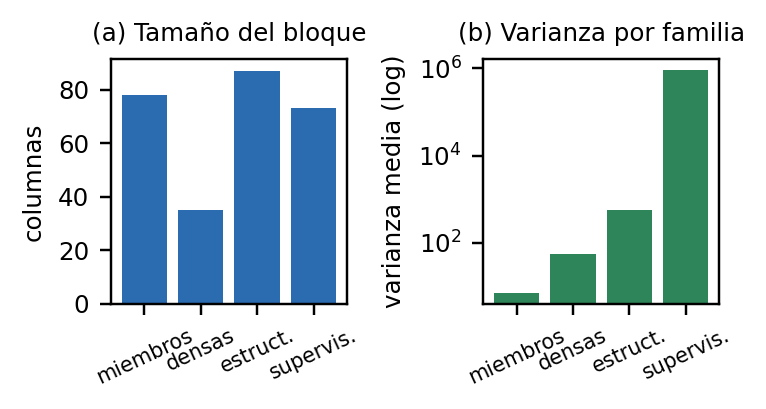
\includegraphics[width=\columnwidth]{figuras/fig_04_bloques.png}
\caption{Tama\~no de cada bloque de la matriz de 279 columnas y varianza media por familia. El bloque supervisado (73 columnas) domina la varianza total y obliga a construirlo dentro de cada fold para no filtrar informaci\'on.}
\label{fig:bloques}
\end{figure}

\begin{figure}[htbp]
\centering
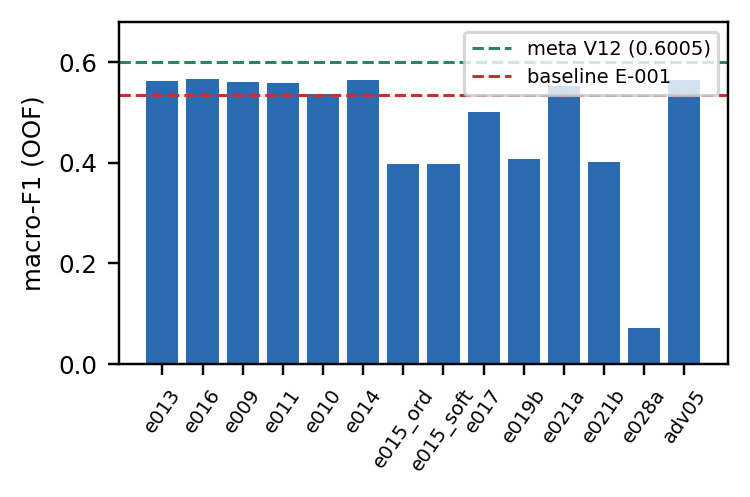
\includegraphics[width=\columnwidth]{figuras/fig_05_miembros.png}
\caption{Aporte individual de los 14 miembros del meta-modelo y su combinaci\'on (V12). La l\'inea verde marca el meta-modelo documentado (0.6005) y la roja el baseline E-001: ninguno de los miembros supera por s\'i solo al meta-modelo; la combinaci\'on de sus probabilidades es la que lo alcanza.}
\label{fig:miembros}
\end{figure}

\begin{table}[htbp]
\centering
\caption{Variables del conjunto de modelado: composici\'on de la matriz de 279 columnas.}
\label{tab:variables}
\footnotesize
\setlength{\tabcolsep}{3pt}
\begin{tabular}{p{0.20\columnwidth}p{0.07\columnwidth}p{0.65\columnwidth}}
\toprule
Bloque & Cols. & Contenido y ejemplos \\
\midrule
Miembros & 78 & Probabilidades (o m\'argenes) fuera de fold de 14 clasificadores individuales, con transformaci\'on logar\'itmica cuando corresponde \\
Densas & 35 & Textometr\'ia estilom\'etrica: longitudes, emoticonos, elongaciones, puntuaci\'on repetida, may\'usculas, d\'igitos, entrop\'ias y ratios de compresi\'on \\
Estructuradas & 87 & Seis familias: distribuci\'on de longitudes, distribuci\'on de caracteres, riqueza l\'exica, forma de palabra, posici\'on y entrop\'ias de puntuaci\'on \\
Supervisadas & 73 & Perfil de clase por entidad (menciones, hashtags, fuente de retuit), rareza l\'exica y l\'exico log-odds por clase, construidas in-fold \\
ADV-07 & 6 & M\'argenes NB-SVM uno-vs-rest de palabra \\
\bottomrule
\end{tabular}
\end{table}

Las variables de origen son m\'inimas: el corpus aporta \'unicamente el identificador, el texto y,
en train, la etiqueta de rango (Tabla~\ref{tab:datos}); no hay metadatos de usuario, fecha ni contadores
sociales, y el identificador se descart\'o como feature tras verificar que su distribuci\'on de
clase es plana. Todo el espacio de variables del modelado se construye a partir del texto y se
organiza en los cinco bloques de la Tabla~\ref{tab:variables}. El bloque de miembros merece
detalle porque fija la diversidad del conjunto: catorce clasificadores de familias distintas
---m\'argenes ordinales de SVM lineales sobre n-gramas de car\'acter y menciones (E-013, E-016,
E-014), regresi\'on log\'istica, SGD y Naive Bayes complementario sobre las mismas
representaciones (E-009, E-011, E-010), una regresi\'on log\'istica sobre n-gramas de palabra
(E-017), una red MLP(256,128) sobre features densas y SVD (E-019b), la familia ordinal de Ridge
y Frank--Hall (E-015, E-021a), centroides de Rocchio (E-021b), SVM de pares adyacentes (E-028a)
y un NB-SVM de car\'acter (ADV-05)---, cuyas probabilidades fuera de fold alimentan el meta con
transformaci\'on logar\'itmica cuando corresponde.

La l\'inea V1-V20 muestra c\'omo se acumul\'o la mejora antes de la fase neuronal. V12, un NB-SVM de palabra con promedio de combinadores (regresi\'on log\'istica y MLP), alcanz\'o 0.6005 de validaci\'on y 0.62182 de \textit{leaderboard}. V19 sum\'o LightGBM \cite{ke2017} como tercer miembro del consenso y subi\'o a 0.6079388 y 0.62578. V20 incorpor\'o la cadena de umbrales anidados y el \textit{blend} de cuatro cuartos \cite{frank2001}, con 0.6097782 y 0.62689. En paralelo, la b\'usqueda de se\~nal residual V13-V17 explor\'o en cinco fases bloques ling\"u\'isticos completos ---morfolog\'ia, lemas, entidades y dependencias---, poda por colinealidad y especialistas de frontera; el mejor bloque ling\"u\'istico aislado rindi\'o 0.2409, muy por encima del azar pero muy por debajo de la representaci\'on vigente, y ninguna de las cinco fases se adopt\'o. Ese resultado, junto con el an\'alisis de la Fig.~\ref{fig:bloques}, dej\'o fijada la estrategia: la se\~nal restante no estaba en features nuevas, sino en c\'omo combinar y c\'omo decidir.

% ===========================================================================
\section{El campe\'on: consenso geom\'etrico de expertos (V48)}
% ===========================================================================

El modelo entregado combina seis componentes de la fase neuronal mediante un \emph{producto de expertos} (PoE). La media aritm\'etica de probabilidades, usada hasta la versi\'on V43, se comporta como un modelo de mezcla con l\'ogica de OR: una confianza espuria de un solo miembro puede desplazar la predicci\'on. El producto de expertos act\'ua como un consenso estricto con l\'ogica de AND, porque penaliza con m\'as fuerza las clases en las que alg\'un experto discrepa \cite{hinton2002,heskes1998}. En un problema con fronteras ordinales tan delicadas, ese comportamiento es el adecuado: el consenso resulta m\'as exigente con el desacuerdo y m\'as estable con el acuerdo. En el relato del proyecto, V48 ocupa el papel de \textbf{ancla p\'ublica} ---el mejor puntaje observado en el \textit{leaderboard}---, mientras que V56, presentado en la Secci\'on~VIII, cumple el papel de \textbf{candidata regularizada} por la mejor validaci\'on local; la selecci\'on conjunta se detalla en esa misma secci\'on.

\subsection{G\'enesis de la arquitectura}

La arquitectura del campe\'on no se dise\~n\'o de una vez. Es el resultado de una cadena de
decisiones, cada una motivada por una pieza del estado del arte y validada por un experimento
sometido a la compuerta pre-registrada del proyecto: una mejora solo se adopta si es positiva en al
menos cuatro de los cinco folds can\'onicos y si el intervalo de confianza pareado excluye el cero.
Esa disciplina explica tanto la forma final del sistema como la ausencia de componentes que, siendo
razonables en teor\'ia, no superaron la medici\'on. La Tabla~\ref{tab:genesis} resume la cadena
completa, con la pieza, su motivaci\'on en la literatura, el experimento que la evalu\'o y la
decisi\'on que se tom\'o.

El punto de partida fue la representaci\'on. El primer experimento (E-001) combin\'o TF-IDF de
n-gramas de car\'acter con un LinearSVC y rindi\'o 0.5344; la incorporaci\'on del canal de
menciones (E-008) elev\'o la l\'inea base hasta 0.5557, y el NB-SVM \cite{wang2012} se consolid\'o
despu\'es como uno de los miembros del meta-modelo. Sobre esa base, el meta-modelo V12 reuni\'o catorce
miembros cl\'asicos y alcanz\'o 0.6005 de validaci\'on local y 0.62182 de \textit{leaderboard}. Ese
resultado fij\'o la hip\'otesis que gui\'o el resto del proyecto: la ganancia no vendr\'ia de una
representaci\'on nueva, sino de la combinaci\'on de miembros diversos y de la decisi\'on sobre el
consenso.

La escalera de validaci\'on local permite seguir la acumulaci\'on de esa ganancia. V19 incorpor\'o
LightGBM \cite{ke2017} como tercer miembro del consenso (0.6079388); V20 a\~nadi\'o la cadena de
umbrales y el \textit{blend} de cuartos ordinales \cite{frank2001} (0.6097782); V30 refin\'o el
\'arbol troncal con Optuna (0.6134471). A partir de ah\'i, el arco neuronal aport\'o incrementos
sucesivos y decrecientes: V38 0.6166579, V39 0.6168017, V40 0.6175912, V41 0.6181119, V42
0.6184162 y V43 0.6184783. El consenso geom\'etrico V48 cerr\'o la escalera con 0.6186451. La
distancia entre el mejor modelo individual con la regla de decisi\'on (V30 con \textit{plug-in},
0.6159732) y el consenso es de $+0.0027$: ese margen, peque\~no en absoluto pero sistem\'atico, es
el valor medido de combinar expertos con sesgos complementarios.

\begin{table*}[htbp]
\centering
\caption{G\'enesis de la arquitectura del campe\'on: cada pieza se adopt\'o despu\'es de un experimento motivado por el estado del arte y validado con la compuerta pre-registrada. La columna de resultado es la macro-F1 de validaci\'on local. Las falsaciones V44--V52 (Secci\'on~\ref{sec:funciono}) descartaron las alternativas y confirmaron que el PoE es el \'optimo de su familia de operadores.}
\label{tab:genesis}
\footnotesize
\setlength{\tabcolsep}{3pt}
\begin{tabular}{p{0.15\textwidth}p{0.33\textwidth}p{0.13\textwidth}p{0.20\textwidth}p{0.14\textwidth}}
\toprule
Pieza & Motivaci\'on en el estado del arte & Experimento & Resultado & Decisi\'on \\
\midrule
Representaci\'on de car\'acter & TF-IDF \textit{char\_wb} (Sapkota); NB-SVM (Wang y Manning) & E-001, E-008 & 0.5344 $\to$ 0.5557 & Base adoptada \\
\'Arbol troncal & LightGBM (Ke et al.) & V19, V20, V29, V30 & 0.6079 $\to$ 0.6134 & Troncal del consenso \\
Red residual tabular & Tabular ResNet (Gorishniy et al.) & V38 & 0.6167 & Adoptada \\
P\'erdida ordinal & Frank--Hall; Wasserstein (Frogner et al.) & V39, V40 & 0.6168, 0.6176 & Adoptada \\
Compuertas SE & Squeeze-and-Excitation (Hu et al.) & V40 & 0.6176 & Adoptadas \\
Promedio de pesos & SWA (Izmailov et al.) & V41 & 0.6181 & Adoptado \\
Suavizado de etiquetas & Szegedy et al.; M\"uller et al. & V42 & 0.6184 & Adoptado \\
Cram\'er sobre la CDF & Cram\'er; von Mises; Sz\'ekely y Rizzo & V43 & 0.6185 & Adoptada \\
Producto de expertos & Hinton; Heskes & V48 & 0.6186 & Campe\'on \\
\textit{Plug-in} por clase & Lipton et al.; Parambath et al. & V30, V48 & $+0.0027$ sobre el consenso & Congelado \\
\bottomrule
\end{tabular}
\end{table*}

La tabla muestra tambi\'en qu\'e se descart\'o. Las falsaciones V44--V52 acotaron el espacio por
exclusi\'on: la distancia $L_1$ de Wasserstein no mejor\'o a Cram\'er (V44); la normalizaci\'on
RankGauss destruy\'o la se\~nal discreta de la matriz (V46); los \'arboles \textit{oblivious} de
CatBoost \cite{prokhorenkova2018} no aportaron al consenso (V49); la atenci\'on multi-cabeza y una
matriz de pesos por clase a\~nadieron varianza sin separaci\'on defendible (V50); la variante
consistente de Cram\'er qued\'o indistinguible de su l\'inea base (V51); y los operadores
intermedios de la familia Power-Mean, las redes autonormalizantes \cite{klambauer2017} y las reglas
por segmento no superaron la compuerta (V52). Ninguna de esas piezas forma parte de V48. Dos de
ellas, V47 y V51, s\'i fueron adoptadas despu\'es como miembros del consenso 2026 (V56), lo que se
declara de forma expl\'icita en la Secci\'on~VIII: una t\'ecnica puede ser insuficiente como modelo
y valiosa como componente.

La lectura conjunta es que la arquitectura final es el \'optimo local de su familia de operadores.
La curva Power-Mean, que interpola entre el producto de expertos y la media aritm\'etica, es
c\'oncava con v\'ertice en $\alpha \to 0$; ning\'un punto intermedio ni la media mejoran al PoE, y
la falsaci\'on V52 lo verific\'o con la compuerta habitual. Cada pieza del campe\'on tiene, por
tanto, trazabilidad completa: una motivaci\'on en el estado del arte, un experimento que la
contrast\'o y un resultado que sostiene la decisi\'on. La especificaci\'on formal que sigue describe
esa arquitectura ya fijada.

\subsection{Formulaci\'on y pesos de los seis expertos}

El consenso se calcula en espacio logar\'itmico como
\begin{equation}
\log P_{\text{geom}}(y = k \mid x) \;\propto\; \sum_{m=1}^{6} w_m \log P_m(y = k \mid x),
\label{eq:poe}
\end{equation}
donde $P_m$ son las probabilidades de cada experto y $w_m$ son pesos no negativos normalizados. La implementaci\'on recorta las probabilidades a $\epsilon = 10^{-12}$ y renormaliza cada fila con la estabilizaci\'on log-sum-exp, de manera que $P_{\text{geom}}$ es una distribuci\'on v\'alida sobre las seis clases. Los pesos se optimizaron por validaci\'on cruzada anidada sobre el s\'implejo, usando exclusivamente los cinco folds can\'onicos agrupados, y convergieron a
\begin{equation}
\mathbf{w}^{\ast} = [0.5628,\; 0.0832,\; 0.1724,\; 0.0754,\; 0.0513,\; 0.0549]
\label{eq:pesos48}
\end{equation}
para los expertos V30, V43, V42, V40, V39-ordinal y V39-HGB, respectivamente. La concentraci\'on del peso en el \'arbol troncal (56.3\%) y en el par de redes con p\'erdida de Cram\'er y suavizado (25.6\% conjunto) refleja sesgos complementarios: los \'arboles de gradiente capturan interacciones discretas de la matriz de features, mientras que las redes ordinales modelan la vecindad entre cohortes.

Los seis expertos son los siguientes. V30 es el LightGBM refinado con Optuna sobre la matriz de 279 columnas \cite{ke2017}, y es el mejor modelo individual del proyecto (0.6134471 de validaci\'on). V43 es una red residual tabular con compuertas Squeeze-and-Excitation \cite{hu2018} entrenada con p\'erdida de Cram\'er $L_2$ sobre la CDF \cite{cramer1928,vonmises1931,szekely2013,frogner2015}, con suavizado de etiquetas \cite{szegedy2016,muller2019} y promedio de pesos estoc\'astico (SWA) \cite{izmailov2018}; V42 usa la misma arquitectura con p\'erdida ordinal suavizada ($\epsilon=0{,}10$). V40 es la variante SE-TabNet con compuertas de excitaci\'on por canal y distancia ordinal esperada, V39-ordinal a\~nade la p\'erdida de entrop\'ia ordinal \cite{frank2001,diaz2019} y V39-HGB es un \textit{HistGradientBoosting} sobre la misma matriz. Las redes comparten la receta general ---AdamW con enfriamiento cosenoidal \cite{loshchilov2017}, entre doce y diecis\'eis \'epocas y SWA en V42/V43---, mientras que V30 y el HGB son ensembles de \'arboles con su propio r\'egimen; la familia completa se evalu\'o antes de combinarse, en el marco de la revisi\'on de redes tabulares de Gorishniy et al.\ \cite{gorishniy2021}. La Tabla~\ref{tab:expertos} detalla la instanciaci\'on de cada experto y la Fig.~\ref{fig:arquitectura} resume la arquitectura completa del campe\'on.

\begin{table*}[htbp]
\centering
\caption{Especificaci\'on de los seis expertos del campe\'on V48. La matriz de 279 columnas es la misma para todos; las redes comparten la receta de entrenamiento (AdamW, lote 256, semillas por fold, promedio de los cinco modelos en test) y solo cambian la p\'erdida y los detalles indicados. Los pesos son los de la ecuaci\'on~(\ref{eq:pesos48}).}
\label{tab:expertos}
\footnotesize
\setlength{\tabcolsep}{4.5pt}
\begin{tabular}{p{0.075\textwidth}>{\raggedright\arraybackslash}p{0.27\textwidth}p{0.235\textwidth}>{\raggedright\arraybackslash}p{0.27\textwidth}p{0.055\textwidth}}
\toprule
Experto & Arquitectura & P\'erdida & Receta & Peso \\
\midrule
V30 & LightGBM: 1.500 \'arboles, 56 hojas, profundidad 7 & Entrop\'ia cruzada multiclase & Optuna anidada (75 pruebas), \textit{early stopping} 60 & 0.5628 \\
V43 & SETabularResNet 279$\to$256$\to$256$\to$256$\to$6; SE $r=4$ & Cram\'er $L_2$ sobre la CDF & AdamW $10^{-3}$, 16 \'epocas, coseno, SWA desde 6 & 0.0832 \\
V42 & SETabularResNet 279$\to$256$\to$256$\to$256$\to$6; SE $r=4$ & Ordinal suavizada ($\epsilon=0{,}10$) & AdamW $10^{-3}$, 16 \'epocas, coseno, SWA desde 6 & 0.1724 \\
V40 & SETabularResNet 279$\to$256$\to$256$\to$256$\to$6; SE $r=4$ & Distancia ordinal esperada & AdamW $10^{-3}$, 12 \'epocas, sin \textit{scheduler} & 0.0754 \\
V39-ord & TabularResNet 279$\to$256$\to$256$\to$256$\to$6 & Entrop\'ia ordinal & AdamW $10^{-3}$, 14 \'epocas, coseno & 0.0513 \\
V39-HGB & HistGradientBoosting & Entrop\'ia cruzada & 300 iteraciones, $\ell_2=1{,}0$ & 0.0549 \\
\bottomrule
\end{tabular}
\end{table*}

El flujo completo del campe\'on es una cadena de cinco etapas sobre una \'unica matriz de 279
columnas: 78 provienen de las probabilidades fuera de fold de los miembros, 35 son densas, 87
estructuradas, 73 supervisadas y 6 son m\'argenes NB-SVM. Esa matriz alimenta a los seis expertos;
cada uno devuelve una distribuci\'on sobre las seis clases; el producto de expertos las combina en
espacio logar\'itmico con los pesos congelados de la ecuaci\'on~(\ref{eq:pesos48}); la regla
\textit{plug-in} por clase reescala el consenso con el vector de la ecuaci\'on~(\ref{eq:plugin}); y
el \textit{argmax} produce la etiqueta final y la \textit{submission} de 112.892 filas. Ninguna
etapa se reajusta sobre el test: los pesos, el vector \textit{plug-in} y la composici\'on del
consenso quedaron congelados antes de generar el env\'io. Los pesos se optimizan por validaci\'on
cruzada anidada sobre el s\'implejo con los cinco folds can\'onicos; el miembro V30 de la
evaluaci\'on publicada usa su predicci\'on fuera de fold de la segunda partici\'on, mientras que la
variante can\'onica rinde 0.6177 y se declara junto al resultado.

La Tabla~\ref{tab:expertos} concreta la instanciaci\'on de esa receta experto por experto. Las
cuatro redes comparten la misma arquitectura interna: \texttt{TabularResNet} proyecta las 279
columnas a 256 dimensiones y encadena dos bloques residuales de 256 unidades con normalizaci\'on por
lotes y activaci\'on SiLU, de modo que cada bloque calcula
$h \leftarrow h + \mathrm{dropout}(\mathrm{SiLU}(\mathrm{BN}(Wh)))$ con una tasa de descarte de
$0{,}2$; la conexi\'on residual preserva la se\~nal de entrada y evita la atenuaci\'on del
gradiente. \texttt{SETabularResNet} intercala una compuerta Squeeze-and-Excitation \cite{hu2018} con
factor de reducci\'on cuatro, que re-pondera las 256 dimensiones de cada bloque antes de la suma
residual, y la cabeza es una capa lineal de 256 a 6. El entrenamiento usa AdamW
\cite{loshchilov2017} con tasa $10^{-3}$ y decaimiento de peso $10^{-4}$, lotes de 256 y entre doce
y diecis\'eis \'epocas seg\'un el experto; V42 y V43 a\~naden enfriamiento cosenoidal hasta
$\eta_{\min}=10^{-4}$ y promedio de pesos estoc\'astico \cite{izmailov2018} desde la \'epoca seis.
Cada red se entrena con la semilla $42+100\cdot\text{fold}$ y, en test, promedia sus cinco modelos;
V39-ordinal y el \textit{HistGradientBoosting} usan un modelo final entrenado sobre todo el
\textit{train}. El \'arbol troncal V30 es un LightGBM \cite{ke2017} de 1.500 \'arboles, 56 hojas,
profundidad 7, tasa $0{,}03$, \texttt{min\_child\_samples} 54, \textit{subsample} $0{,}78$,
\textit{colsample} $0{,}6$, $\alpha=0{,}015$, $\lambda=0{,}0005$ y parada temprana de 60
iteraciones, con el espacio de b\'usqueda fijado por la Optuna anidada de 75 pruebas.

\begin{figure*}[htbp]
\centering
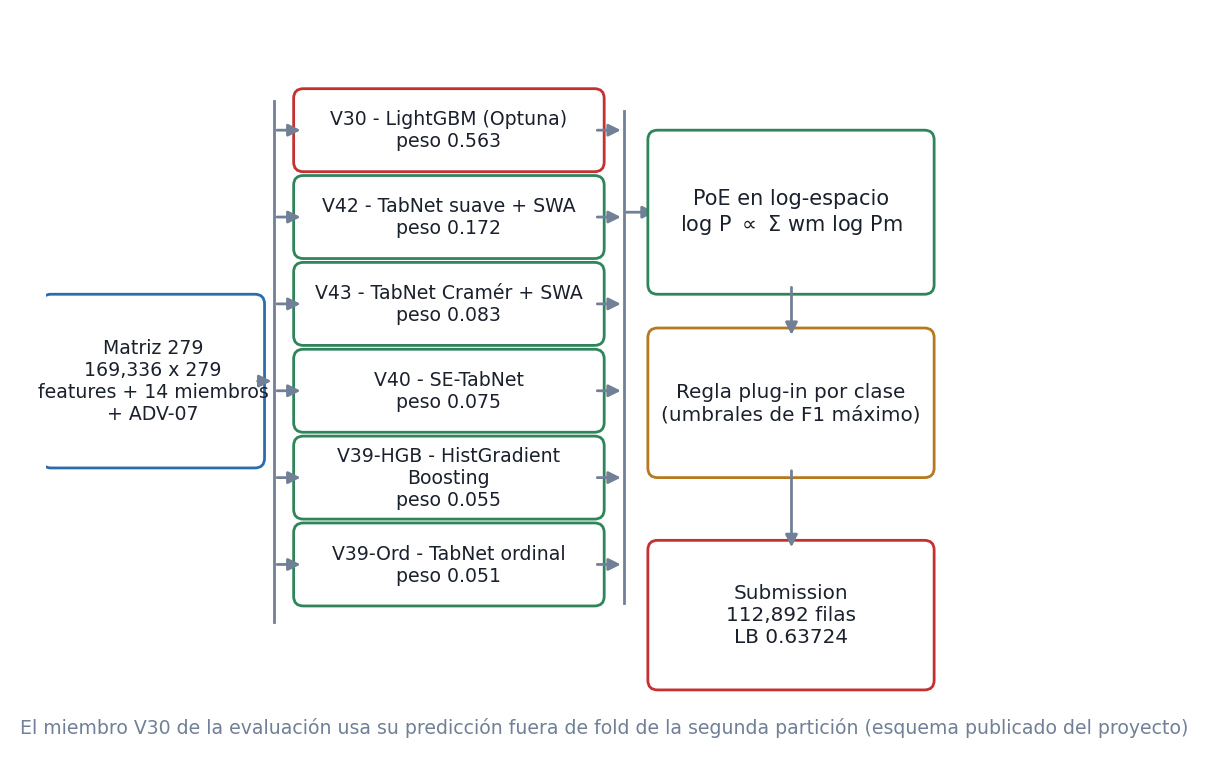
\includegraphics[width=0.88\textwidth]{figuras/fig_arquitectura_v48.png}
\caption{Arquitectura del campe\'on V48. La matriz de 279 columnas alimenta seis expertos con sesgos complementarios ---dos ensembles de \'arboles y cuatro redes tabulares con p\'erdidas ordinales--- cuyas probabilidades se combinan en espacio logar\'itmico con los pesos de la ecuaci\'on~(\ref{eq:pesos48}); sobre el consenso se aplica la regla \textit{plug-in} congelada y se genera la \textit{submission} de 112.892 filas. El miembro V30 de la evaluaci\'on usa su predicci\'on fuera de fold de la segunda partici\'on, seg\'un el esquema publicado del proyecto.}
\label{fig:arquitectura}
\end{figure*}

La elecci\'on del operador geom\'etrico proviene de una caracterizaci\'on completa de la familia de operadores de consenso. La familia Power-Mean,
\begin{equation}
P_\alpha(y = k \mid x) \;\propto\; \Big( \sum_{m=1}^{M} w_m \, P_m(y = k \mid x)^{\alpha} \Big)^{1/\alpha},
\label{eq:powermean}
\end{equation}
interpola entre el producto de expertos ($\alpha \to 0$) y la media aritm\'etica ($\alpha = 1$). La curva medida sobre las predicciones fuera de fold es c\'oncava con v\'ertice en $\alpha = 0$: la media aritm\'etica degrada $-0.000208$ con 0/5 folds positivos, el \textit{rank-averaging} colapsa $-0.02257$ porque destruye la densidad continua que la regla de decisi\'on necesita, y los puntos intermedios quedan por debajo del v\'ertice. El PoE es, por tanto, el \'optimo de su familia, como qued\'o registrado en la falsaci\'on V52.

\subsection{Resultado y verificaci\'on estad\'istica}

El consenso con la regla de decisi\'on alcanz\'o \textbf{0.6186451 de macro-F1 en validaci\'on local} y \textbf{0.63724 en el \textit{leaderboard} de Kaggle} (referencia 57283487), el mejor puntaje del proyecto. Dos precisiones hacen verificable el resultado. La primera: el esquema publicado ---con el que se report\'o el resultado--- usa para el miembro V30 su predicci\'on fuera de fold de la \emph{segunda partici\'on}; la variante estricta con el V30 can\'onico rinde 0.6177 y se reporta de forma expl\'icita. La segunda: la mejora sobre el campe\'on aritm\'etico anterior (V43) se someti\'o a la compuerta pre-registrada ---4 de 5 folds positivos, con el quinto virtualmente id\'entico ($-0.000008$), y bootstrap pareado con intervalo de confianza al 95\% de $[+0.0000007, +0.0004095]$ que excluye el cero ($p = 0.0250$)---; el env\'io cambi\'o 290 filas del test (0.26\%).

La ablaci\'on cualitativa del consenso a\'isla el aporte de cada bloque. Sin el \'arbol troncal V30 el consenso pierde del orden de 0.006 de macro-F1, una magnitud que ning\'un miembro individual puede compensar; y los miembros neuronales, que individualmente rinden entre 0.6086 y 0.6132 (Fig.~\ref{fig:neuronal}), aportan el resto de la mejora sobre la l\'inea V30 con \textit{plug-in} (0.6159732): aproximadamente $+0.0027$. La lectura es consistente con el resto del proyecto: el valor de las redes no est\'a en su desempe\~no aislado, sino en la diversidad de sus errores frente al \'arbol.

\subsection{La regla \textit{plug-in} sobre el consenso}

Sobre el consenso geom\'etrico se aplica la regla de decisi\'on calibrada por clase descrita en la Secci\'on~IV,
\begin{equation}
\hat{y}(x) = \arg\max_{k \in \{1,\dots,6\}} \; w^{\text{plug}}_k \cdot P_{\text{geom}}(y = k \mid x),
\label{eq:decision}
\end{equation}
con el vector congelado de la ecuaci\'on~(\ref{eq:plugin}). La Tabla~\ref{tab:plugin} muestra su efecto por clase sobre las predicciones fuera de fold. La regla sube la macro-F1 global moviendo decisiones hacia las clases infra-predichas: 18-24 gana $+0.0064$, 65-xx $+0.0065$ y 25-34 $+0.0019$, mientras que 13-17 cede $-0.0045$ de F1 porque era la clase sobre-predicha y financia con ese sacrificio el equilibrio global. El patr\'on de recall confirma el mecanismo: la regla eleva el recall de 25-34 en $+0.044$ y el de 18-24 en $+0.021$, y lo reduce en las cohortes extremas, donde el modelo ya decid\'ia con precisi\'on alta. Como se\~nala la teor\'ia de umbralizaci\'on \'optima de F-medidas \cite{lipton2014,parambath2014,waegeman2014,narasimhan2015,eban2017}, la exactitud global baja mientras la m\'etrica objetivo sube: es la firma de un cambio de regla de decisi\'on, no de representaci\'on.

\begin{table}[htbp]
\centering
\caption{Efecto de la regla \textit{plug-in} por clase sobre las predicciones fuera de fold (169.336 filas): F1 con \textit{argmax} y con la regla, recall con la regla y filas predichas por clase.}
\label{tab:plugin}
\begin{tabular}{lccccc}
\toprule
Rango & F1 \textit{argmax} & F1 \textit{plug-in} & $\Delta$F1 & Recall & $n$ pred. \\
\midrule
13-17 & 0.6854 & 0.6809 & $-0.0045$ & 0.6192 & 23.634 \\
18-24 & 0.5208 & 0.5273 & $+0.0064$ & 0.5699 & 33.311 \\
25-34 & 0.4992 & 0.5011 & $+0.0019$ & 0.5203 & 30.518 \\
35-49 & 0.5731 & 0.5738 & $+0.0006$ & 0.5508 & 25.968 \\
50-64 & 0.6671 & 0.6682 & $+0.0011$ & 0.6940 & 30.232 \\
65-xx & 0.7351 & 0.7416 & $+0.0065$ & 0.7213 & 25.673 \\
\bottomrule
\end{tabular}
\end{table}

\subsection{An\'alisis de error y calibraci\'on validaci\'on-\textit{leaderboard}}

La Fig.~\ref{fig:confusion} muestra la matriz de confusi\'on y el F1 por clase del campe\'on sobre las predicciones fuera de fold. El patr\'on es exactamente el que la estructura ordinal del problema predice: los extremos se clasifican mejor ---65-xx alcanza 0.745 de F1 y 13-17 llega a 0.685--- y los rangos centrales concentran el error, con 25-34 en 0.505 y 18-24 en 0.531. Las confusiones se concentran en las fronteras adyacentes, que es lo que las p\'erdidas de Cram\'er y la cadena de umbrales est\'an dise\~nadas a favorecer, y los errores lejanos son marginales. La Fig.~\ref{fig:progresion} completa la lectura con la progresi\'on hasta la regla \textit{plug-in} y con la estructura de probabilidad condicional por rango real: la diagonal es n\'itida y las celdas vecinas absorben la masa restante.

\begin{figure*}[htbp]
\centering
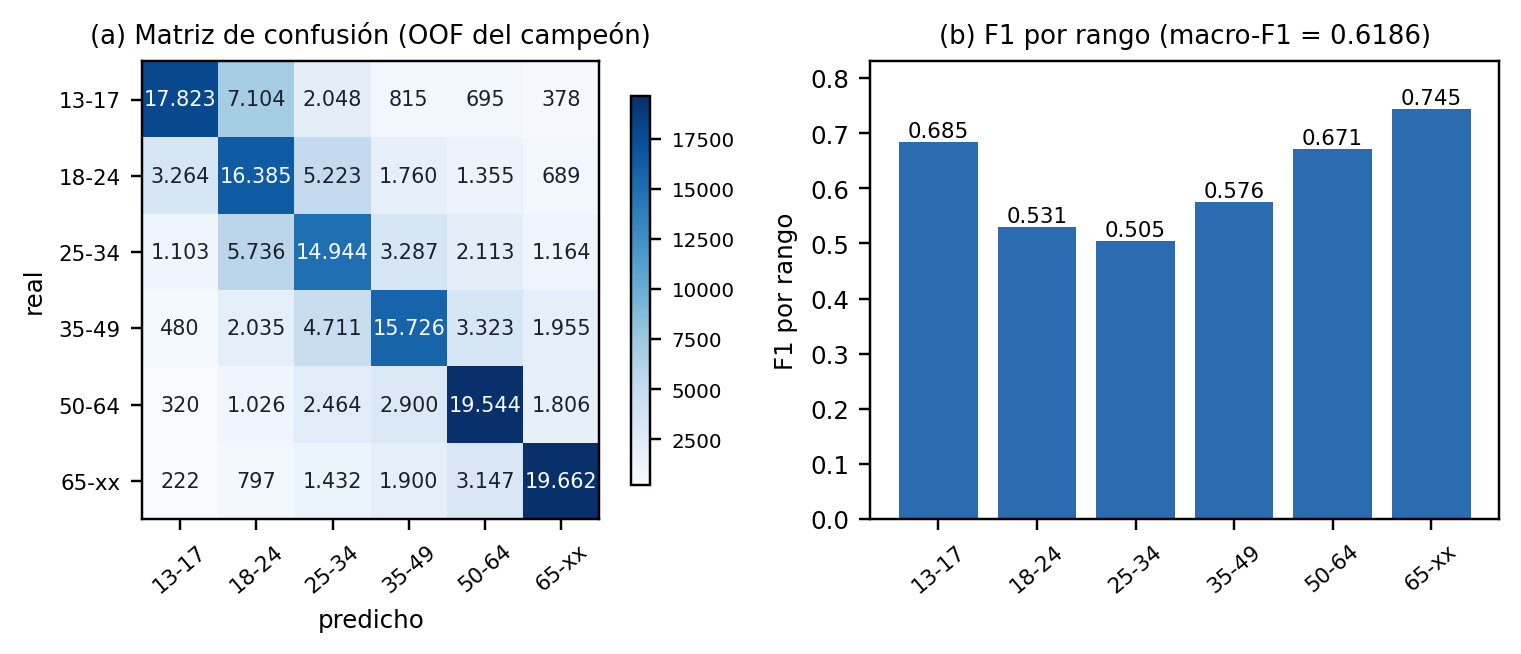
\includegraphics[width=0.92\textwidth]{figuras/fig_07_confusion.png}
\caption{Matriz de confusi\'on y F1 por rango del campe\'on (predicciones fuera de fold). Los extremos 13-17 y 65-xx se clasifican mejor (0.685 y 0.745) y los rangos centrales concentran el error (18-24: 0.531; 25-34: 0.505) por solapamiento de vocabulario entre cohortes vecinas.}
\label{fig:confusion}
\end{figure*}

\begin{figure}[htbp]
\centering
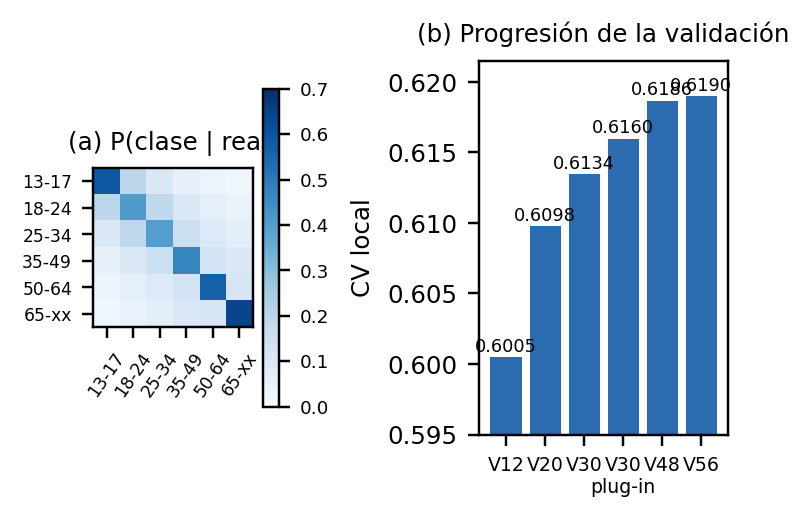
\includegraphics[width=\columnwidth]{figuras/fig_08_progresion.png}
\caption{Estructura de la decisi\'on del campe\'on. Izquierda: probabilidad media por clase condicionada al rango real sobre la predicci\'on del modelo troncal, con la diagonal dominante. Derecha: progresi\'on de la validaci\'on desde V12 hasta la regla \textit{plug-in}; cada eslab\'on a\~nade un mecanismo distinto (representaci\'on, ordinalidad, optimizaci\'on y decisi\'on).}
\label{fig:progresion}
\end{figure}

Por \'ultimo, la calibraci\'on entre validaci\'on local y \textit{leaderboard} cierra el cuadro: la brecha del campe\'on es de $+0.0186$ (0.63724 frente a 0.6186451), consistente con la brecha hist\'orica del proyecto ($+0.0177 \pm 0.0023$) y explicada, como se argument\'o en la Secci\'on~III, por la memorizaci\'on de \textit{near-duplicados} del test. La brecha del campe\'on es consistente con la escalera completa de versiones. La Fig.~\ref{fig:evolucion} sit\'ua esa brecha frente al techo declarado del dato, que se discute en la Secci\'on~VII.

\begin{figure*}[htbp]
\centering
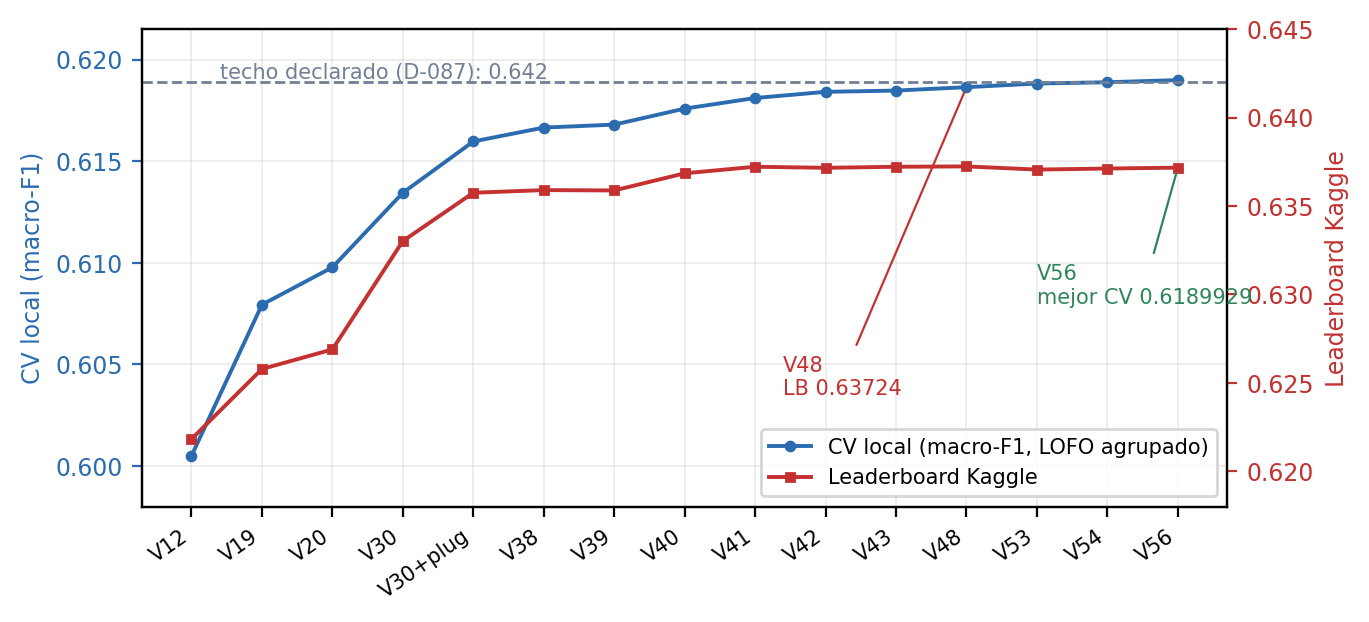
\includegraphics[width=0.88\textwidth]{figuras/fig_evolucion.png}
\caption{Evoluci\'on de la validaci\'on local (macro-F1, leave-one-fold-out agrupado) y del \textit{leaderboard} de Kaggle a lo largo de las versiones del proyecto. La l\'inea discontinua marca el techo declarado del dato (0.642, Decisi\'on 5). La curva local es sistem\'aticamente inferior a la del \textit{leaderboard} por la memorizaci\'on de \textit{near-duplicados} del test, y la distancia entre ambas es estable, lo que valida la calibraci\'on CV-\textit{leaderboard}.}
\label{fig:evolucion}
\end{figure*}

% ===========================================================================
\section{Qu\'e funcion\'o y qu\'e no}
\label{sec:funciono}
% ===========================================================================

\subsection{Lo que funcion\'o}

Cinco mecanismos concentraron todas las adopciones del proyecto. Primero, la representaci\'on NB-SVM con n-gramas de car\'acter \cite{wang2012,mukherjee2010,sapkota2013,sapkota2015}, que sostuvo la versi\'on V12 (0.6005 de validaci\'on, 0.62182 de \textit{leaderboard}) y nunca fue desplazada como base. Segundo, el \textit{boosting} con la cadena de umbrales anidados \cite{ke2017,frank2001}, que llev\'o la l\'inea a V19 y V20 (0.6079388 y 0.6097782). Tercero, la optimizaci\'on de hiperpar\'ametros con Optuna sobre la matriz de 279 columnas, que produjo V30 con una ganancia de $+0.0037$ y convirti\'o al \'arbol troncal en el miembro dominante de todos los consensos posteriores. Cuarto, la regla de decisi\'on \textit{plug-in} por clase \cite{lipton2014}, cuyo aporte de $+0.0025$ result\'o mayor que el de cualquier arquitectura nueva de la fase final: el proyecto aprendi\'o que decidir mejor con el modelo existente era m\'as rentable que reemplazarlo. Quinto, las redes tabulares con p\'erdidas ordinales, suavizado de etiquetas y SWA \cite{gorishniy2021,cramer1928,szegedy2016,izmailov2018,hu2018}, que escalaron la validaci\'on de 0.6167 a 0.6185 entre V38 y V43 y culminaron en el consenso geom\'etrico V48.

\begin{figure}[htbp]
\centering
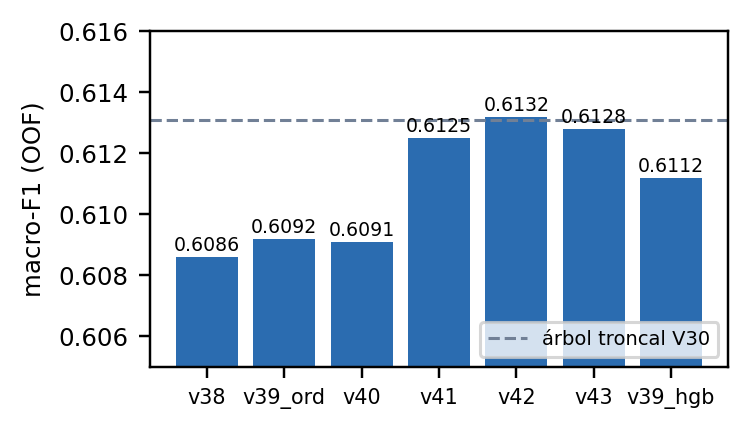
\includegraphics[width=\columnwidth]{figuras/fig_10_familia_nn.png}
\caption{Desempe\~no individual de la familia neuronal (V38-V43) y del \textit{HistGradientBoosting} sobre la matriz de 279 columnas. Ninguna red supera por s\'i sola al \'arbol troncal (l\'inea discontinua, 0.6131), pero su diversidad de errores es lo que el consenso geom\'etrico explota.}
\label{fig:neuronal}
\end{figure}

\subsection{Las falsaciones documentadas}

El registro de lo que no funcion\'o es igualmente informativo. El proyecto cerr\'o la b\'usqueda de se\~nal residual V13-V17 con cinco fases sin adopciones ---bloques ling\"u\'isticos completos, poda por colinealidad, arquitecturas de combinador y especialistas de frontera--- y las versiones V44 a V52 con ocho falsaciones adicionales, todas medidas con el mismo protocolo y la misma compuerta pre-registrada. La Tabla~\ref{tab:falsaciones} resume las seis m\'as informativas, con la hip\'otesis, el resultado exacto y la conclusi\'on transferible.

\begin{table*}[htbp]
\centering
\caption{Falsaciones clave: hip\'otesis, resultado medido y conclusi\'on. Todas se evaluaron con el protocolo can\'onico y la compuerta pre-registrada (consistencia por folds e intervalo de confianza pareado que excluya el cero).}
\label{tab:falsaciones}
\begin{tabular}{p{0.26\textwidth}p{0.34\textwidth}p{0.34\textwidth}}
\toprule
Hip\'otesis & Resultado medido & Conclusi\'on \\
\midrule
Bloques ling\"u\'isticos completos (morfolog\'ia, lemas, entidades y dependencias) aportar\'ian se\~nal al meta-modelo (V13-V17) & Mejor bloque aislado 0.2409 (azar 0.1667); fusi\'on $-0.0015$ (1/5 folds); poda por colinealidad $-0.0040$ (0/5) & Una representaci\'on puede tener se\~nal real en aislamiento y no aportar nada al integrarse: el modelo existente ya la expresa mejor \\
Penalizar las fronteras con distancia $L_1$ (Wasserstein-1) destrabar\'ia el cuello de botella (V44) & OOF 0.6183063, $\Delta = -0.0001720$ frente a V43; 1/5 folds; $p = 0.8550$ & Los gradientes discontinuos de $L_1$ oscilan alrededor del umbral \'optimo; la distancia cuadr\'atica de Cram\'er es estrictamente superior \\
Normalizar por cuantiles (RankGauss) eliminar\'ia los picos de gradiente de una matriz muy asim\'etrica (V46) & Standalone 0.6055514, el peor de la familia neuronal; en consenso $\Delta = -0.0000327$; 2/5 folds & Forzar distribuciones cero-infladas hacia una normal destruye la se\~nal discreta del indicador de ausencia \\
Los \'arboles sim\'etricos de CatBoost capturar\'ian patrones globales del segmento sin menci\'on (V49) & Standalone 0.6066473; PoE de 7 con $\Delta = -0.0000816$; 2/5 folds; $p = 0.7480$ & Los \'arboles \textit{oblivious} no rescatan la se\~nal del segmento sin menciones ni aportan al consenso \\
La atenci\'on multi-cabeza sobre tokens sint\'eticos y una matriz de pesos por clase mejorar\'ian las fronteras (V50) & MHSA 0.6073432 en fold 0; sustituci\'on de la rama SE: $-0.0005204$; matriz $W$ nominal $+0.0000474$ con $p = 0.1940$ & La atenci\'on carece del sesgo inductivo localizado de las compuertas SE, y estimar 36 par\'ametros en lugar de 6 a\~nade varianza sin separaci\'on defendible \\
Operadores intermedios de la familia Power-Mean, redes autonormalizantes y reglas por segmento mejorar\'ian el consenso (V52) & $\alpha = 0.5$: $-0.000242$ y $\alpha = 1.0$: $-0.000208$ (0/5 folds); SNN $-0.00913$; regla por segmento: $-0.0013763$ & El PoE geom\'etrico es el \'optimo de su familia, y la m\'etrica arm\'onica no admite reglas por segmento sin romper la calibraci\'on marginal (paradoja de Simpson) \\
\bottomrule
\end{tabular}
\end{table*}

Dos falsaciones merecen un comentario adicional. La de las reglas por segmento (V52) se apoya en la paradoja de Simpson \cite{simpson1951}: subir el F1 del segmento sin menciones en $+0.000185$ hundi\'o la macro-F1 global en $-0.0013763$, porque los falsos positivos y falsos negativos de ambos segmentos se suman en el mismo denominador. Y la bater\'ia V45 ---21 hip\'otesis pre-registradas de discretizaci\'on, compuertas, \textit{meta-arbitraje} y reoptimizaci\'on del \textit{plug-in}--- no produjo ninguna mejora: la peor variante, la discretizaci\'on unidimensional, perdi\'o $-0.04167$, y hasta la reoptimizaci\'on del vector \textit{plug-in} dentro de los folds result\'o contraproducente ($-0.0003374$), lo que confirma que los pesos congelados no estaban inflados.

El detalle de las mediciones ilustra el criterio. En la b\'usqueda residual V13-V17 se probaron
bloques ling\"u\'isticos completos (morfolog\'ia, lemas, entidades y dependencias de un
analizador externo), poda por colinealidad (58 cl\'usteres que cubren 171 de 310 variables;
$-0.0040$ reproducible en dos particiones), arquitecturas de combinador y especialistas de
frontera: el mejor bloque aislado rindi\'o 0.2409, muy por encima del azar (0.1667) pero muy por
debajo de la representaci\'on vigente, y ninguna de las cinco fases super\'o la compuerta. Las mediciones de la segunda familia (V44-V52) est\'an tabuladas en la Tabla~\ref{tab:falsaciones}, con su hip\'otesis, resultado y conclusi\'on.

\subsection{V47 y V51: falsaciones individuales con adopci\'on posterior}

Dos falsaciones merecen un comentario aparte. V47 (Cram\'er asim\'etrico ponderado con recorte de valores at\'ipicos) y V51 (Cram\'er consistente suavizado) fallaron como modelos individuales: V47 no pas\'o la compuerta con 3/5 folds y $p = 0.2620$, y V51 qued\'o indistinguible de su l\'inea base ($\Delta = -0.0000302$ en el consenso de reemplazo, $p = 0.6900$). Sin embargo, ambas fueron \textbf{adoptadas como miembros del consenso 2026} (Secci\'on~VIII), porque su se\~nal d\'ebil result\'o complementaria en el espacio logar\'itmico. La conclusi\'on es matizada: una t\'ecnica puede ser insuficiente como modelo y valiosa como componente, y la forma de determinarlo es medir la contribuci\'on marginal dentro del consenso, no el desempe\~no aislado.

\subsection{El techo declarado del dato}

El l\'imite se estableci\'o por medici\'on. La Decisi\'on 5 fij\'o el techo alcanzable en \textbf{0.642 de macro-F1 en el \textit{leaderboard}} y refut\'o el objetivo de 0.70 con un argumento de informaci\'on disponible: alcanzarlo exigir\'ia una validaci\'on local del orden de 0.6786, es decir $+0.0626$ sobre el campe\'on, mientras que un or\'aculo restringido a la misma informaci\'on que el modelo ya tiene ---corregir solo las filas donde la probabilidad de la clase verdadera supera un umbral $\tau$--- rinde como m\'aximo $+0.0568$ en $\tau = 0.30$ y decae r\'apidamente despu\'es. Dicho de otro modo: incluso un corrector perfecto que solo usara la informaci\'on que el campe\'on ya posee se quedar\'ia corto. El residuo medido respalda la conclusi\'on: el 38.62\% de las filas queda mal clasificado, y de esos errores el 59.94\% es de distancia ordinal uno, es decir, confusiones entre cohortes vecinas que la b\'usqueda de se\~nal residual V13-V17 y las falsaciones V44-V52 ya hab\'ian intentado explotar sin \'exito. La b\'usqueda qued\'o saturada y el techo qued\'o establecido.

% ===========================================================================
\subsection{Inventario del espacio experimental}

El espacio completo de experimentaci\'on queda contabilizado en \textbf{220 filas}: 171 ejecutadas,
26 documentales, 12 pre-registros, 10 enmiendas y 1 bloqueada. La Tabla~\ref{tab:lineas} las agrupa
en diecis\'eis l\'ineas de trabajo, con el rango de resultados de cada una y su veredicto; el
Ap\'endice~\ref{ap:catalogo} lista los 220 identificadores con su macro-F1 de validaci\'on local. El
detalle fila a fila ---pregunta, hip\'otesis, medici\'on y decisi\'on--- vive en el cat\'alogo del
proyecto (\texttt{experiments.csv}, \texttt{RUNLOG.md} y \texttt{DECISIONS.md}), reproducible de
extremo a extremo.

\begin{table*}[htbp]
\centering
\caption{L\'ineas de experimentaci\'on del cat\'alogo (220 experimentos) con su resultado agregado. Los identificadores de cada l\'inea y su macro-F1 individual est\'an en el Ap\'endice~\ref{ap:catalogo}.}
\label{tab:lineas}
\footnotesize
\setlength{\tabcolsep}{3pt}
\begin{tabular}{p{0.175\textwidth}p{0.065\textwidth}p{0.04\textwidth}p{0.345\textwidth}p{0.315\textwidth}}
\toprule
L\'inea & Bloque & $n$ & Resultado (macro-F1) & Veredicto \\
\midrule
Representaci\'on y l\'inea base & B2 & 18 & 0.4971--0.5557; \texttt{E-008} 0.5557 & TF-IDF de car\'acter y NB-SVM adoptados \\
Modelos cl\'asicos y miembros & B3 & 12 & 0.3381--0.5851; \texttt{E-020} 0.5851 & Catorce miembros para el meta-modelo \\
Features avanzadas & B4 & 7 & 0.5641--0.5966; \texttt{ADV-03} 0.5966 & \texttt{ADV-07} entra en la matriz \\
Fases PH y meta-modelo & B5 & 30 & 0.5906--0.6108; V12 0.6005 & El meta-modelo supera a sus miembros \\
Canales l\'exicos & B6 & 5 & 0.2033--0.6004 & Sin adopci\'on \\
V13--V15, ling\"u\'istica & B7--8 & 19 & mejor bloque aislado 0.2409 & Falsado: sin adopci\'on \\
V16--V18, meta-arquitectura & B9--11 & 16 & 0.5990--0.6011; \texttt{V16} 0.6011 & La se\~nal restante no est\'a en features nuevas \\
V19--V22, ordinalidad & B12--17 & 19 & V19 0.6079; V20 0.6098 & V20 entra en el linaje; V21--V22 sin adopci\'on \\
V23--V29, selecci\'on y Optuna & B18--23 & 12 & \texttt{V29} 0.6122; CORAL 0.4837 & Optuna fija el espacio del troncal \\
V30--V31, campe\'on y canales & B24 & 9 & V30 0.6134; \texttt{V31-ENS-N1} 0.6139 & Troncal definitivo; canales sin adopci\'on \\
Auditor\'ia y \textit{plug-in} & B25--29 & 6 & 0.6155 can\'onica; 0.6165 alterna & Regla \textit{plug-in} congelada y adoptada \\
V32--V37, \textit{challengers} & B30--37 & 42 & 0.1721--0.6149; ninguna supera el troncal & FTRL, CatBoost, MLP-surrogate y canales ling\"u\'isticos cerrados \\
V38--V43, arco neuronal & B38--43 & 6 & 0.6167--0.6185; \texttt{V43} 0.6185 & Cinco componentes adoptados \\
V44--V52, falsaciones & B44--52 & 9 & 0.6183--0.6187 & Solo V48: el PoE es el \'optimo de su familia \\
V53--V57, frontera 2026 & B53--57 & 5 & 0.6182--0.6190; \texttt{V56} 0.6190 & R\'ecord local y auditor\'ia del s\'implejo \\
Auditor\'ia final & B99 & 5 & cinco acciones, sin modelo & Cierre verificable del historial \\
\midrule
\textbf{Total} & & \textbf{220} & & \\
\bottomrule
\end{tabular}
\end{table*}

El recorrido de la tabla reproduce la historia del sistema. La l\'inea de representaci\'on (B2) se
mueve entre 0.4971 y 0.5557 y entrega la base de TF-IDF de car\'acter y el canal de menciones; los modelos
cl\'asicos (B3) llegan a 0.5851 y aportan catorce miembros al meta-modelo; las features avanzadas
(B4) suben a 0.5966 con \texttt{ADV-03} y dejan \texttt{ADV-07} en la matriz; y las fases PH con
el meta-modelo (B5) cierran en 0.6108, con V12 en 0.6005. La b\'usqueda ling\"u\'istica
(B6--B8) es el primer l\'imite claro: el mejor bloque aislado rindi\'o 0.2409 ---por encima del
azar de 0.1667, pero muy por debajo de la representaci\'on vigente--- y ninguna de sus variantes se
adopt\'o. La meta-arquitectura V16--V18 (B9--B11) se qued\'o en 0.5990--0.6011 y confirm\'o que la
se\~nal restante no estaba en features nuevas.

La ordinalidad y la selecci\'on movieron la aguja. V19 y V20 (B12--B17) llevaron la validaci\'on a
0.6079 y 0.6098; V25--V29 (B18--B23) se movieron entre 0.6092 y 0.6122 y fijaron con Optuna el
espacio del \'arbol troncal; V30 (B24) alcanz\'o 0.6134 y, con la regla \textit{plug-in} congelada,
0.6160. Los \textit{challengers} V32--V37 (B30--B37) exploraron FTRL, CatBoost, sustitutos de MLP
y canales ling\"u\'isticos hasta 0.6149, sin superar al troncal. El arco neuronal V38--V43
(B38--B43) escal\'o de 0.6167 a 0.6185 y aport\'o los cinco componentes que el consenso adopt\'o.

Las falsaciones V44--V52 (B44--B52) se concentraron en una banda estrecha, 0.6183--0.6187, y solo
V48 se adopt\'o; la frontera 2026 V53--V57 (B53--B57) lleg\'o a 0.6182--0.6190, con V56 como
r\'ecord local, y las auditor\'ias de cierre (B99) no produjeron modelo sino verificaci\'on del
historial. La lectura es que la mejora se concentra en cuatro mecanismos ---representaci\'on,
ordinalidad, combinaci\'on y decisi\'on--- y que las 220 filas delimitan emp\'iricamente el espacio:
fuera de esas cuatro palancas, ninguna de las familias restantes movi\'o la m\'etrica m\'as all\'a
de las mil\'esimas.

\section{La frontera 2026 y la auditor\'ia matem\'atica}
% ===========================================================================

Tras el resultado de V48, el proyecto sigui\'o empujando la frontera con tres piezas nuevas ---una arquitectura densa multi-escala, dos variantes del transporte ordinal de Cram\'er y un \'arbol sim\'etrico--- m\'as una auditor\'ia matem\'atica del consenso. La pregunta era si el espacio logar\'itmico admit\'ia miembros a\'un m\'as diversos sin degradar las cohortes minoritarias; la respuesta qued\'o medida: el techo de validaci\'on local subi\'o a \textbf{0.6189929} (V56, 5/5 folds positivos, $p = 0.0010$ frente a V48) y la \textbf{selecci\'on dual V48/V56} qued\'o ratificada como n\'ucleo de la entrega final.

\subsection{V53: la red densa y el consenso de siete modelos}

La red densa conecta cada bloque con todos los siguientes ($192 \to 320 \to 448 \to 576$) para preservar las representaciones tempranas sin diluci\'on aditiva \cite{huang2017}, con compuertas Squeeze-and-Excitation \cite{hu2018} y la p\'erdida de Cram\'er consistente suavizada \cite{cramer1928,szekely2013}. Como clasificador individual rinde 0.6111343 ---por debajo de las redes residuales, que promedian 0.6128--- pero integrada al consenso geom\'etrico de siete modelos con la regla \textit{plug-in} congelada alcanza \textbf{0.6188259} de validaci\'on (4/5 folds positivos, $p = 0.0280$) y \textbf{0.63706} en Kaggle. El diagn\'ostico de su transferencia fue instructivo: asignar un peso no amortiguado ($w = 0.025$) a una red de calidad individual inferior contrajo la cohorte 13-17 al 13.76\% de las predicciones, frente al 17.04\% de prevalencia real.

\subsection{V54: la unificaci\'on jer\'arquica de Cram\'er}

V54 corrigi\'o ese desequilibrio con un ensamble jer\'arquico: la rama de transporte ordinal fusiona 0.80 de Cram\'er sim\'etrico (V43) con 0.20 de Cram\'er asim\'etrico ponderado y winsorizado a $[-6, +6]$ (V47), y la red densa queda amortiguada en $w = 0.0200$. El resultado es \textbf{0.6188887} de validaci\'on (4/5 folds, $p = 0.0050$, intervalo de confianza $[+0.0000599, +0.0004324]$) y \textbf{0.63712} en Kaggle, con solo 180 filas cambiadas respecto de V48 (0.16\%). La restauraci\'on del equilibrio marginal en las cohortes minoritarias fue el mecanismo identificable de la mejora.

\subsection{V55: el octa-modelo limpio y la protecci\'on de la evaluaci\'on privada}

Al constatar que las redes densas rinden por debajo de las residuales en aislamiento, V55 excluy\'o formalmente las arquitecturas sub\'optimas e inyect\'o un \'arbol sim\'etrico CatBoost con peso 0.00805 \cite{prokhorenkova2018} en un consenso de ocho modelos de m\'axima calidad individual. Rindi\'o 0.6182436 de validaci\'on (4/5 folds frente a V48) y \textbf{0.63707} en Kaggle, y se adopt\'o como protocolo de protecci\'on para la evaluaci\'on privada: la idea era que una \textit{submission} construida solo con miembros de calidad demostrada deber\'ia degradarse menos que sus competidoras cuando el 30\% privado del \textit{leaderboard} entre en juego.

\subsection{V56: el consenso no lineal de nueve modelos}

V56 integr\'o en un solo consenso nueve modelos de sesgos ortogonales: el \'arbol troncal V30 ($w = 0.5594$), las redes V42 ($0.1687$), V40 ($0.0608$), V43 ($0.0602$), V39-ordinal ($0.0438$) y V39-HGB ($0.0520$), y los tres miembros del arco 2026: la red densa V53 ($0.0238$), el Cram\'er asim\'etrico V47 ($0.0209$) y el Cram\'er consistente V51 ($0.0104$). El resultado es la \textbf{mejor validaci\'on local del proyecto: 0.6189929 de macro-F1}, con 5/5 folds positivos frente a V54 ($+0.000078$, $+0.000005$, $+0.000115$, $+0.000249$ y $+0.000079$), un bootstrap pareado frente a V48 con $p = 0.0010$ e intervalo $[+0.0001485, +0.0005590]$ estrictamente positivo, y \textbf{0.63717 en Kaggle} (referencia 57350295). La \textit{submission} de V56 difiere de la del campe\'on en solo 194 filas de 112.892 (0.17\%): la mejora es real pero delgada, y esa delgadez es precisamente lo que exige la verificaci\'on estad\'istica de la Secci\'on~IX. La Tabla~\ref{tab:hitos} recorre los once hitos de la evoluci\'on completa.

\begin{table*}[htbp]
\centering
\caption{Hitos de la evoluci\'on: mecanismo, validaci\'on local (macro-F1, leave-one-fold-out agrupado) y \textit{leaderboard} de Kaggle. Las cifras de V48 y V56 corresponden al mejor \textit{leaderboard} y a la mejor validaci\'on local del proyecto, respectivamente.}
\label{tab:hitos}
\begin{tabular}{llccc}
\toprule
Versi\'on & Mecanismo & CV local & LB Kaggle & Nota \\
\midrule
V12 & NB-SVM + promedio de LogReg y MLP & 0.6005000 & 0.62182 & Baseline del meta-modelo \\
V19 & + LightGBM como tercer miembro & 0.6079388 & 0.62578 & El \textit{boosting} entra al consenso \\
V20 & Cuartos + cadena de umbrales anidados & 0.6097782 & 0.62689 & Ordinalidad explotada \\
V30 & Optuna sobre la matriz de 279 columnas & 0.6134471 & 0.63302 & Mejor modelo individual del proyecto \\
V30 + \textit{plug-in} & Regla de decisi\'on por clase & 0.6159732 & 0.63575 & $+0.0025$ por decidir mejor \\
V41 & \textit{Blend} aritm\'etico con SWA-SE & 0.6181119 & 0.63722 & Primera mejora de SWA \\
V43 & \textit{Blend} aritm\'etico Cram\'er-SWA & 0.6184783 & 0.63722 & \'Ultimo \textit{blend} aritm\'etico adoptado \\
\textbf{V48} & \textbf{PoE geom\'etrico de 6 expertos} & \textbf{0.6186451} & \textbf{0.63724} & \textbf{Mejor puntaje del proyecto en \textit{leaderboard}} \\
V53 & PoE de 7 con red densa & 0.6188259 & 0.63706 & Mejor validaci\'on hasta V54 \\
V54 & PoE de 8 con Cram\'er unificado & 0.6188887 & 0.63712 & Mejor validaci\'on hasta V56 \\
\textbf{V56} & \textbf{PoE de 9 modelos} & \textbf{0.6189929} & \textbf{0.63717} & \textbf{Mejor validaci\'on local del proyecto} \\
\bottomrule
\end{tabular}
\end{table*}

\subsection{La auditor\'ia matem\'atica V57}

El cierre del arco fue una auditor\'ia matem\'atica sobre las predicciones fuera de fold de V56, con cuatro an\'alisis que en conjunto caracterizan la cuenca de generalizaci\'on del consenso.

\emph{Sensibilidad en el s\'implejo.} Se perturb\'o cada uno de los nueve pesos en $\pm 20\%$ y se reevalu\'o el consenso. Todos los modelos resultan estacionarios: cualquier variaci\'on produce $\Delta \le 0$ con $|\Delta F1| \le \sim 4 \times 10^{-4}$, y las perturbaciones m\'as costosas son las del \'arbol troncal y de la red de suavizado, coherentes con sus pesos. No hay ninguna coordenada cuya subida mejore el \'optimo.

\emph{Concavidad de la familia Power-Mean.} La curva de la ecuaci\'on~(\ref{eq:powermean}) para $\alpha \in [-0.15, +0.15]$ es c\'oncava con v\'ertice \'unico en $\alpha = 0$, el PoE, y decae suavemente hacia ambos lados ($-1.4 \times 10^{-4}$ en $\alpha = -0.15$ y $-2.9 \times 10^{-5}$ en $\alpha = +0.15$). El \'optimo de la familia no est\'a en un borde: est\'a exactamente en el operador adoptado, y la superficie es plana en su entorno, lo que explica la robustez del consenso frente a la elecci\'on fina de pesos.

\emph{Confiabilidad decil a decil.} Ordenando las 169.336 predicciones por confianza y agrup\'andolas en diez deciles, la exactitud es estrictamente mon\'otona y coincide con la confianza media: el decil inferior promedia 0.278 de confianza y 0.268 de exactitud, y el superior 0.992 y 0.995. El modelo est\'a bien calibrado en todo el rango, sin sobreconfianza ni zonas muertas.

\emph{La brecha de menciones.} El 63.9\% de los tweets contiene una menci\'on y se clasifica mucho mejor (exactitud 0.6802, confianza 0.6863, brecha de 0.0060) que el 36.1\% sin menci\'on (0.4997 y 0.5004, brecha de 0.0007). Este resultado tiene una explicaci\'on directa: la menci\'on activa las features estructuradas y el bloque supervisado del segmento, y su ausencia deja al modelo con la se\~nal puramente estil\'istica. Lo relevante es que ambas ramas est\'an autocalibradas, lo que explica por qu\'e las reglas desacopladas por segmento de V52 fallaban: el problema no era de calibraci\'on, sino de agregaci\'on de la m\'etrica \cite{simpson1951}.

A la auditor\'ia se sum\'o una falsaci\'on adicional: optimizar una p\'erdida sustituta continua (log-loss multiclase en validaci\'on anidada) en lugar de la m\'etrica objetivo degrada el resultado a 0.6186997 ($\Delta = -0.0002932$, 0/5 folds positivos), porque la superficie del log-loss sesga los pesos hacia los \'arboles de decisi\'on y se desalinea de la macro-F1. Las Figs.~\ref{fig:powermean} y~\ref{fig:v57} muestran las dos piezas centrales de la auditor\'ia.

\begin{figure}[htbp]
\centering
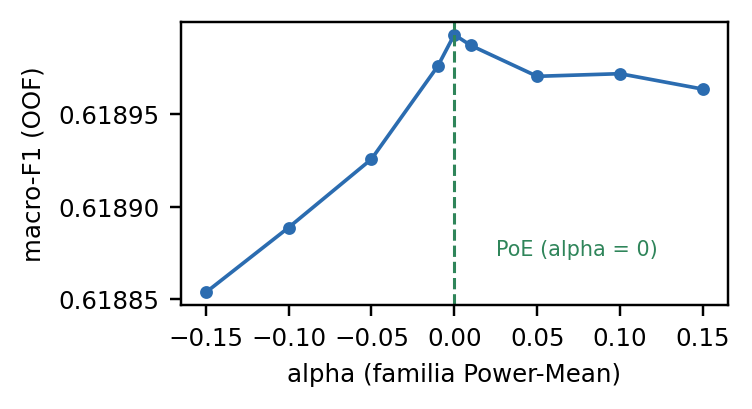
\includegraphics[width=\columnwidth]{figuras/fig_11_powermean.png}
\caption{Concavidad de la familia Power-Mean del consenso V56 sobre las predicciones fuera de fold (auditor\'ia V57). El v\'ertice \'unico est\'a en $\alpha = 0$, es decir, en el producto de expertos: la media aritm\'etica ($\alpha = 1$) y todos los operadores intermedios quedan por debajo.}
\label{fig:powermean}
\end{figure}

\begin{figure*}[htbp]
\centering
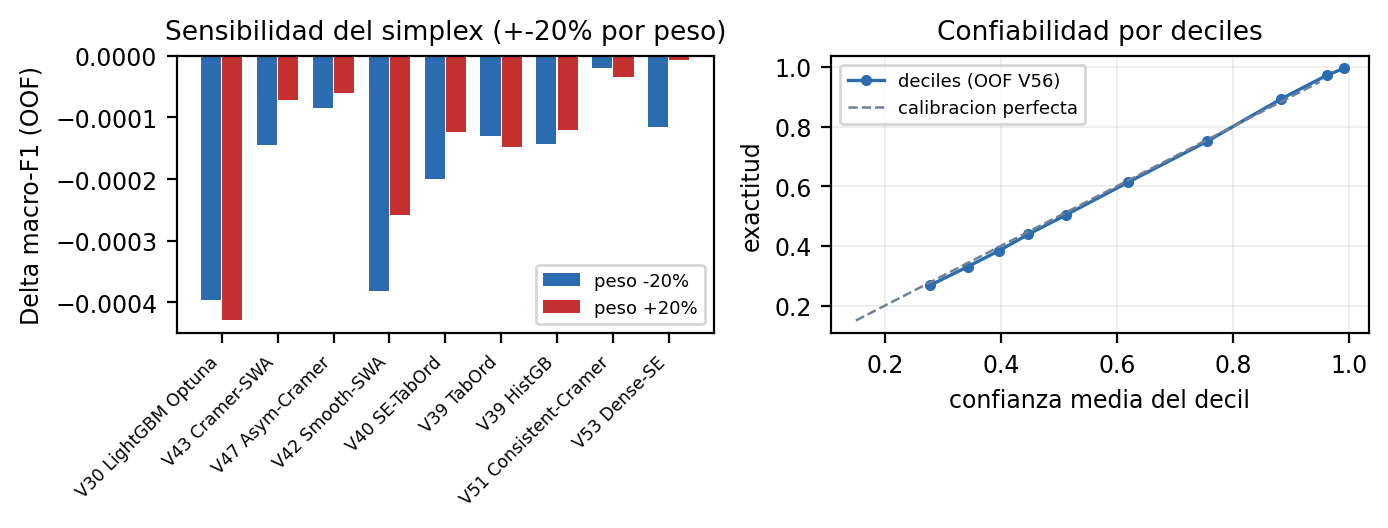
\includegraphics[width=0.95\textwidth]{figuras/fig_v57_analisis.png}
\caption{Auditor\'ia matem\'atica del consenso V56. Izquierda: sensibilidad del s\'implejo de nueve pesos ante perturbaciones de $\pm 20\%$ por coordenada; todas las perturbaciones degradan la m\'etrica, luego la soluci\'on es un \'optimo estacionario. Derecha: confiabilidad decil a decil sobre las 169.336 predicciones fuera de fold, con exactitud estrictamente mon\'otona y pegada a la diagonal de calibraci\'on perfecta.}
\label{fig:v57}
\end{figure*}

\subsection{La selecci\'on dual ante la evaluaci\'on privada}

La auditor\'ia no cambi\'o la \textit{submission}: respald\'o la decisi\'on. La calificaci\'on final de la competencia depende en un 70\% del 30\% privado del \textit{leaderboard}, que permanece oculto hasta el cierre, y la parte alta de la tabla estaba separada por mil\'esimas. La plataforma de Kaggle permite seleccionar un portafolio de hasta diez env\'ios para la evaluaci\'on final. Lejos de usarlo para ensayar variantes aleatorias, el proyecto articul\'o un portafolio estratificado encabezado por su \textbf{selecci\'on dual nuclear}: V48 como ancla p\'ublica ---mejor puntaje observado, 0.63724, con su \textit{submission} enviada--- y V56 como candidata de m\'axima regularizaci\'on ---mejor validaci\'on local, 5/5 folds positivos, $p = 0.0010$, con \textit{submission} propia de 194 filas distintas---, respaldado por las soluciones intermedias de la frontera (V54, V43, V41 y V30 + \textit{plug-in}), que cubren las posibles desviaciones distributivas del 30\% privado sin dispersar el foco metodol\'ogico. La auditor\'ia V57 mostr\'o que ambas soluciones habitan un \'optimo estacionario, inmune al sobreajuste del \textit{leaderboard} p\'ublico, y la Decisi\'on 11 fij\'o el techo estacionario y descart\'o el ajuste especulativo posterior sobre el \textit{leaderboard}. El criterio se mantuvo desde la primera fase: las decisiones se toman sobre validaci\'on, el \textit{leaderboard} se usa para calibrar y el cierre se respalda estad\'isticamente.

% ===========================================================================
\section{Validaci\'on estad\'istica}
% ===========================================================================

\subsection{Significancia de las mejoras del arco 2026}

Las mejoras del arco 2026 frente al campe\'on son del orden de tres diezmil\'esimas de macro-F1, una magnitud dif\'icil de interpretar por s\'i sola: en un problema de seis clases casi balanceadas y 169.336 filas de evaluaci\'on, cualquier diferencia peque\~na puede ser fruto del azar de la partici\'on. Por eso cada adopci\'on se someti\'o a un \emph{bootstrap pareado} con 1.000 remuestreos sobre las predicciones fuera de fold, remuestreando cl\'usteres de \textit{near-duplicados} en lugar de filas sueltas para preservar la dependencia entre textos casi id\'enticos, y exigiendo que el intervalo de confianza al 95\% de la diferencia excluyera el cero. La Tabla~\ref{tab:significancia} resume el resultado: V53 alcanza $p = 0.0280$ ---bordeando el cero en su cota inferior, con 4/5 folds---, mientras que V54 ($p = 0.0050$) y V56 ($p = 0.0010$) consolidan intervalos de confianza al 95\% estrictamente positivos, este \'ultimo con 5/5 folds favorables. La consistencia por folds acompa\~na la significancia: V56 supera a V54 en los cinco folds (+0.000078, +0.000005, +0.000115, +0.000249 y +0.000079), y V53 y V54 lo hacen en cuatro de cinco. Una mejora de $+0.0003$ con 5/5 folds y $p = 0.0010$ es peque\~na pero real, del orden de lo que cabe esperar cuando el sistema opera cerca del techo del dato.

\begin{table}[htbp]
\centering
\caption{Significancia de las mejoras del arco 2026 frente al campe\'on V48 (bootstrap pareado, $B = 1.000$, sobre las predicciones fuera de fold; intervalos de confianza al 95\%).}
\label{tab:significancia}
\footnotesize
\setlength{\tabcolsep}{3.5pt}
\begin{tabular}{lcccc}
\toprule
Versi\'on & $\Delta$CV & Folds $+$ & $p$ & IC95 \\
\midrule
V53 & $+0.000181$ & 4/5 & 0.0280 & $[-0.0000024,+0.0003684]$ \\
V54 & $+0.000244$ & 4/5 & 0.0050 & $[+0.0000599,+0.0004324]$ \\
V56 & $+0.000348$ & 5/5 & 0.0010 & $[+0.0001485,+0.0005590]$ \\
\bottomrule
\end{tabular}
\end{table}

El balance final del proyecto es de 220 experimentos registrados, cero errores de auditor\'ia de idioma y auditor\'ias formales de fugas de informaci\'on y de formato de la \textit{submission} superadas. La Fig.~\ref{fig:test} cierra el ciclo con la distribuci\'on final de decisiones sobre el test.

\begin{figure}[htbp]
\centering
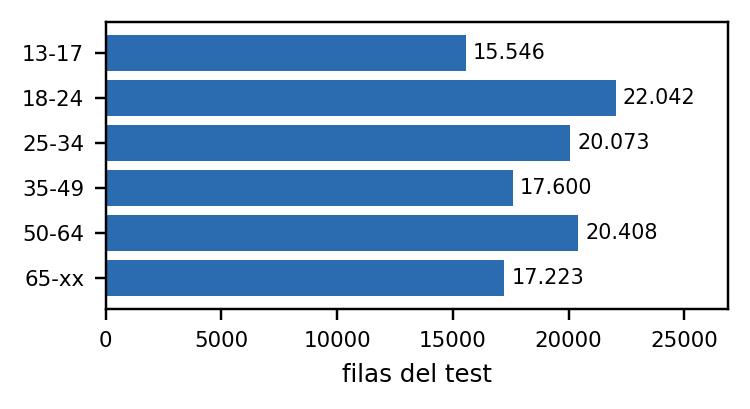
\includegraphics[width=\columnwidth]{figuras/fig_13_test.png}
\caption{Distribuci\'on final de las decisiones sobre las 112.892 filas del test para la \textit{submission} del campe\'on. Las seis clases quedan representadas en proporciones cercanas a la prevalencia del entrenamiento; las desviaciones reflejan el efecto conjunto del modelo y de la regla de decisi\'on por clase.}
\label{fig:test}
\end{figure}

% ===========================================================================
\section{Discusi\'on y limitaciones}
% ===========================================================================

La evidencia acumulada sostiene una tesis central: \textbf{el techo observado es del dato, no del modelo}. Tres propiedades del corpus lo explican. Primero, la redundancia interna es alta: el diagn\'ostico de la matriz midi\'o un factor de inflaci\'on de varianza mediano de 18.87, con 170 variables por encima de 10 y 58 cl\'usteres de colinealidad que cubren 171 de 310 variables, mientras que 87 de 278 direcciones concentran el 95\% de la varianza; a\~nadir features nuevas a ese espacio rara vez aporta algo que las existentes no expresen ya. Segundo, el vocabulario de cohortes vecinas se solapa casi por completo, como muestra el an\'alisis l\'exico de la Secci\'on~III, de modo que el 59.94\% del error residual es de distancia ordinal uno: confusiones entre rangos contiguos que ninguna de las t\'ecnicas probadas ---especialistas de frontera, distancias asim\'etricas, atenci\'on, reglas por segmento--- logr\'o convertir en mejoras estables. Tercero, no hay metadatos: sin usuario, fecha ni red social, la \'unica se\~nal es textual, y la menci\'on es el \'unico rasgo estructural fuerte (el 63.9\% de los tweets con menci\'on se clasifica a 0.680 de exactitud, frente a 0.500 del resto). La b\'usqueda de se\~nal residual qued\'o saturada tras 27 variantes controladas, y el techo declarado en 0.642 de macro-F1 en el \textit{leaderboard} resume el l\'imite medido.

El riesgo de \textit{shakeup} condicion\'o la estrategia final. La calificaci\'on de la competencia depende en un 70\% del 30\% privado del \textit{leaderboard}, invisible hasta el cierre, y la parte alta de la tabla estaba separada por mil\'esimas. El proyecto opt\'o por no perseguir el puntaje p\'ublico y proteger la decisi\'on final: la auditor\'ia V57 mostr\'o que el consenso habita un \'optimo estacionario, con calibraci\'on mon\'otona decil a decil y sin coordenadas del s\'implejo que mejoren la soluci\'on, y la selecci\'on dual V48/V56 ---ancla p\'ublica y candidata regularizada--- dej\'o la decisi\'on final en manos de la evidencia local. El criterio fue el mismo de todo el proyecto: decidir sobre validaci\'on y usar el \textit{leaderboard} solo para calibrar.

Las limitaciones del trabajo se declaran sin matices. El corpus est\'a transliterado a ASCII, de modo que la se\~nal de tildes y emojis ---documentada como \'util en la literatura de perfilado--- es inaccesible por construcci\'on del dataset, no por decisi\'on del equipo. Las reglas de la competencia prohibieron \textit{transformers}, \textit{embeddings} y LLM, as\'i que los resultados no son comparables con el estado del arte neuronal en perfilado de autor; lo que este trabajo mide es, precisamente, cu\'anto se puede lograr sin esas herramientas. No se usaron datos externos etiquetados, por decisi\'on \'etica del equipo, y la procedencia del corpus es desconocida: no hay manera de verificar c\'omo se recolect\'o ni de agrupar por autor, que ser\'ia el protocolo \'optimo para la validaci\'on y para el modelado. La segunda partici\'on de validaci\'on comparte filas con la primera ---solape parcial declarado---, de modo que sirve como verificaci\'on de robustez, no como evaluaci\'on independiente. Y la brecha sistem\'atica entre validaci\'on y \textit{leaderboard} implica que las cifras de Kaggle no son comparables con las locales: la honestidad de este art\'iculo consiste en reportar ambas y explicar la diferencia.

% ===========================================================================
\section{Conclusiones}
% ===========================================================================

La pregunta de investigaci\'on admite ahora una respuesta directa. \textbf{El PLN cl\'asico alcanza 0.63724 de macro-F1 en el \textit{leaderboard} p\'ublico}: un consenso geom\'etrico de seis expertos cl\'asicos ---\'arboles de gradiente, redes tabulares con comprensi\'on ordinal del problema y una regla de decisi\'on calibrada por clase--- logra ese puntaje, $+0.08489$ sobre el baseline inicial. \textbf{Y el techo del dato est\'a medido}: 0.642 en el \textit{leaderboard} como m\'aximo alcanzable bajo las restricciones vigentes, con el objetivo de 0.70 refutado mediante el argumento de informaci\'on disponible y con la b\'usqueda residual saturada tras 220 experimentos. Entre ambos extremos queda un sistema que sube a lo largo de la escalera completa ---representaci\'on, ordinalidad, optimizaci\'on, combinaci\'on y decisi\'on--- y que establece su mejor validaci\'on local en 0.6189929 con nueve modelos, 5/5 folds positivos y $p = 0.0010$ frente al campe\'on.

Tres pr\'acticas quedan como recomendaci\'on general. La primera es la \textbf{validaci\'on agrupada por \textit{near-duplicados}}: sin ella, el baseline de memorizaci\'on pasa de 0.0000 a 0.0608 de macro-F1 y cada decisi\'on de modelo se toma sobre se\~nal inflada; en corpus sociales con contenido replicado, agrupar es un requisito del protocolo. La segunda es la \textbf{separaci\'on estricta entre ajuste, validaci\'on y \textit{leaderboard}}, con calibraci\'on expl\'icita de la brecha entre ellos: el proyecto midi\'o $+0.0177 \pm 0.0023$ y la us\'o para leer cada env\'io contra una expectativa cuantificada. La tercera es la \textbf{selecci\'on en portafolio}: la plataforma permite elegir hasta diez env\'ios para la evaluaci\'on final, y el proyecto la aprovech\'o con criterio ---una candidata anclada en el mejor puntaje observado, otra regularizada por la mejor validaci\'on local y las soluciones intermedias de la frontera---, todas decididas con el mismo protocolo estad\'istico. En conjunto, cuando el modelo se acerca al techo del dato, la ventaja competitiva se traslada de la arquitectura al protocolo: c\'omo se valida, c\'omo se decide y c\'omo se verifica.

% ===========================================================================
\section*{Ap\'endice A. Cat\'alogo completo de experimentos}
\addcontentsline{toc}{section}{Ap\'endice A. Cat\'alogo completo de experimentos}
\phantomsection
\newcounter{apendicecatalogo}
\renewcommand{\theapendicecatalogo}{A}
\refstepcounter{apendicecatalogo}
\label{ap:catalogo}
\begingroup\raggedright

El cat\'alogo del proyecto contiene las 220 filas de experimentaci\'on que sostienen este art\'iculo.
Se listan aqu\'i todas, agrupadas por bloque de trabajo y en orden cronol\'ogico, con su macro-F1 de
validaci\'on local cuando existe. La daga ($^{\dagger}$) marca los experimentos sin una \'unica m\'etrica
agregada ---pre-registros, enmiendas, auditor\'ias, estudios multi-brazo y documentales--- cuyo
resultado, cuando procede, se discute en el cuerpo del art\'iculo. Los bloques de trabajo se corresponden con
las l\'ineas de la Tabla~\ref{tab:lineas}; el bloque B99 re\'une las auditor\'ias de cierre.

\par\medskip\noindent\textbf{B2 · representaci\'on y l\'inea base (18).} \texttt{E-001} 0.5344; \texttt{E-002a} 0.5025; \texttt{E-002b} 0.4971; \texttt{E-002c} 0.4941; \texttt{E-003a} 0.5262; \texttt{E-003b} 0.5408; \texttt{E-003c} 0.5413; \texttt{E-005a} 0.3902; \texttt{E-007a} 0.5339; \texttt{E-005b} 0.4107; \texttt{E-005c} 0.5277; \texttt{E-005d} 0.4094; \texttt{E-005e} 0.5264; \texttt{E-004b} 0.5354; \texttt{E-008} 0.5557; \texttt{B0} 0.0485; \texttt{B1} 0.5015; \texttt{B5} 0.3568.

\par\medskip\noindent\textbf{B3 · modelos cl\'asicos y miembros (12).} \texttt{E-009} 0.5603; \texttt{E-010} 0.5370; \texttt{E-011} 0.5579; \texttt{E-012} 0.5624; \texttt{E-014} 0.5644; \texttt{E-015} 0.3973; \texttt{E-016} 0.5658; \texttt{E-017} 0.5015; \texttt{E-018} 0.5784; \texttt{E-019a} 0.3381; \texttt{E-019b} 0.4071; \texttt{E-020} 0.5851.

\par\medskip\noindent\textbf{B4 · features avanzadas (7).} \texttt{ADV-01}$^{\dagger}$; \texttt{ADV-02} 0.5897; \texttt{ADV-03} 0.5966; \texttt{ADV-04} 0.5899; \texttt{ADV-05} 0.5641; \texttt{ADV-06} 0.5904; \texttt{ADV-07} 0.5867.

\par\medskip\noindent\textbf{B5 · fases PH y meta-modelo V12 (30).} \texttt{PH1-L1} 0.5906; \texttt{PH2-L6} 0.5967; \texttt{PH3-V11} 0.6024; \texttt{PH5-L2} 0.5948; \texttt{PH6-L3} 0.5975; \texttt{PH7-L7} 0.6005; \texttt{PH8-V12} 0.6077; \texttt{PH9-COMB} 0.6005; \texttt{PH10-A} 0.5987; \texttt{PH10-B} 0.5944; \texttt{PH11-RUIDO} 0.6020; \texttt{PH12-AUD} 0.6004; \texttt{PH13-ERR} 0.6005; \texttt{PH14-CONS} 0.6002; \texttt{PH15-CALIB} 0.6007; \texttt{PH15B-SUBSETS} 0.6004; \texttt{PH18-LIMPIEZA} 0.6013; \texttt{PH16-ORD-GREEDY} 0.6001; \texttt{PH21-VISTA} 0.6022; \texttt{PH22-VISTA2} 0.6010; \texttt{PH19-HOLDOUT-VISTA} 0.6108; \texttt{PH24-DIAG}$^{\dagger}$; \texttt{PH25-FRESCA}$^{\dagger}$; \texttt{PH26-ESTABILIDAD}$^{\dagger}$; \texttt{PH27-V12REPRO}$^{\dagger}$; \texttt{PH30-COBERTURA}$^{\dagger}$; \texttt{PH31-DECISION} 0.6015; \texttt{PH32-CORRECCION} 0.6006; \texttt{PH33-CORRECTOR} 0.6000; \texttt{PH34-INFORME-DEC} 0.6005.

\par\medskip\noindent\textbf{B6 · canales l\'exicos (5).} \texttt{PH36-COBERTURA-LEX}$^{\dagger}$; \texttt{PH37-CATALOGO-LEX}$^{\dagger}$; \texttt{PH38-BLOQUES-LEX} 0.2033; \texttt{PH39-FUSION-LEX} 0.6004; \texttt{PH40-ANALISIS-ERROR-LEX}$^{\dagger}$.

\par\medskip\noindent\textbf{B7--B8 · V13--V15, b\'usqueda ling\"u\'istica (19).} \texttt{V13-P0A-IDIOMA}$^{\dagger}$; \texttt{V13-P0B-COLINEALIDAD}$^{\dagger}$; \texttt{V13-P1C-IDENTIDADES} 0.3997; \texttt{V13-P1A-TOKENS} 0.3997; \texttt{V13-P17A-PRONOMBRES} 0.1918; \texttt{V13-P17B-PRONOMBRES} 0.1922; \texttt{V13-P20-MODALIDAD} 0.1270; \texttt{V13-P1B-FUSION} 0.6003; \texttt{V13-P16-SUFIENCIA} 0.0485; \texttt{V13-P16B-ACTIVACION}$^{\dagger}$; \texttt{V13-P16C-RECONSTRUCCION} 0.0485; \texttt{V13-P16D-PUERTA} 0.6005; \texttt{V13-P3A-ESPECIALISTAS} 0.5993; \texttt{V13-P19-CONJUNCIONES} 0.1539; \texttt{V13-CIERRE}$^{\dagger}$; \texttt{V14A-LINGUISTICO} 0.2409; \texttt{V14B-FUSION-LINGUISTICO} 0.5990; \texttt{V15A-CORRELACION}$^{\dagger}$; \texttt{V15B-PODA} 0.5965.

\par\medskip\noindent\textbf{B9--B11 · V16--V18, meta-arquitectura y frontera (16).} \texttt{V16-ARQUITECTURA} 0.6011; \texttt{V17-P0-AUDITORIA}$^{\dagger}$; \texttt{V17-P0-REPRODUCCION} 0.6011; \texttt{V17-P1-FRONTERAS}$^{\dagger}$; \texttt{V17-P1B-CURVA} 0.6007; \texttt{V17-P8-CONFIANZA}$^{\dagger}$; \texttt{V17-P1C-CONJUNTA} 0.6005; \texttt{V17-P9-ARBITRO} 0.6004; \texttt{V17-P5-COMBINADOR} 0.6003; \texttt{V18-P0-AUDITORIA}$^{\dagger}$; \texttt{V18-P0-REPRODUCCION} 0.6005; \texttt{V18-P1-PESO-CLASES} 0.6001; \texttt{V18-P3-MARGEN} 0.5990; \texttt{V18-P4-MULTIOBJETIVO} 0.5993; \texttt{V18-P5-DESTILACION}$^{\dagger}$; \texttt{V18-CIERRE}$^{\dagger}$.

\par\medskip\noindent\textbf{B12--B17 · V19--V22, ordinalidad (19).} \texttt{AGE-CIERRE-AUDITORIA}$^{\dagger}$; \texttt{AGE-DECISION-EJECUTIVA}$^{\dagger}$; \texttt{V19-B1-BOOSTING}$^{\dagger}$; \texttt{V19-B1-VERIFICACION}$^{\dagger}$; \texttt{V19-B1-CONFIRMACION}$^{\dagger}$; \texttt{V19-B1-CHALLENGER}$^{\dagger}$; \texttt{V19-P0-AUDITORIA}$^{\dagger}$; \texttt{V19-X1-EXPLOTACION}$^{\dagger}$; \texttt{V20-AUDIT}$^{\dagger}$; \texttt{V20-F1-CLASECOND}$^{\dagger}$; \texttt{V20-F2-CLASEFUNC}$^{\dagger}$; \texttt{V20-F3-UMBRALES}$^{\dagger}$; \texttt{V20-F3C-CANDIDATO}$^{\dagger}$; \texttt{V20-P2-PESOS}$^{\dagger}$; \texttt{V21-B1-ESPECIALISTA}$^{\dagger}$; \texttt{V22-ORDINAL-COMPARTIDO}$^{\dagger}$; \texttt{V22-B1-SPECIALIST}$^{\dagger}$; \texttt{V22-00-FRONTIER}$^{\dagger}$; \texttt{V22-01-COSTE-ORDINAL}$^{\dagger}$.

\par\medskip\noindent\textbf{B18--B23 · V23--V29, selecci\'on y Optuna (12).} \texttt{V23-00-TESTS-CORAL} 0.9781; \texttt{V23-01-CORAL} 0.4837; \texttt{V25-00-INVENTARIO}$^{\dagger}$; \texttt{V25-01-SELECCION-MI} 0.6092; \texttt{V26-00-GAP-ANALYSIS}$^{\dagger}$; \texttt{V26-01-REPRESENTACION} 0.6098; \texttt{V27-01} 0.6098; \texttt{V27-02} 0.6094; \texttt{V27-05} 0.6101; \texttt{V28-02} 0.6095; \texttt{V28-03} 0.5422; \texttt{V29-01} 0.6122.

\par\medskip\noindent\textbf{B24 · V30--V31, campe\'on y canales (9).} \texttt{V30-01} 0.6122; \texttt{V31-00} 0.6134; \texttt{V31-01}$^{\dagger}$; \texttt{V31-02} 0.4987; \texttt{V31-03} 0.5048; \texttt{V31-04} 0.5048; \texttt{V31-ENS-N1} 0.6139; \texttt{V31-ENS-N2} 0.6117; \texttt{V31-J}$^{\dagger}$.

\par\medskip\noindent\textbf{B25--B29 · auditor\'ia y regla \textit{plug-in} (6).} \texttt{G14-AUDIT}$^{\dagger}$; \texttt{AUDIT-COVERAGE}$^{\dagger}$; \texttt{AGE-CLOSURE}$^{\dagger}$; \texttt{AGE-PLUGIN-CANON} 0.6155; \texttt{AGE-PLUGIN-ALT} 0.6165; \texttt{AGE-PLUGIN-SUBMISSION}$^{\dagger}$.

\par\medskip\noindent\textbf{B30--B37 · V32--V37, \textit{challengers} y canales ling\"u\'isticos (42).} \texttt{AGE-PLUGIN-ADOPTED}$^{\dagger}$; \texttt{AGE-LING-P0-GAP}$^{\dagger}$; \texttt{AGE-LING-P1-LEGALITY}$^{\dagger}$; \texttt{AGE-LING-RESOLUTION}$^{\dagger}$; \texttt{AGE-LING-P2-PREREG}$^{\dagger}$; \texttt{AGE-LING-P2-POS-SEQ} 0.6073; \texttt{AGE-LING-P6-PREREG}$^{\dagger}$; \texttt{AGE-LING-P6-NER}$^{\dagger}$; \texttt{AGE-LING-P7-PREREG}$^{\dagger}$; \texttt{AGE-LING-P7-TYPED}$^{\dagger}$; \texttt{AGE-LING-REMAINING-PREREG}$^{\dagger}$; \texttt{AGE-LING-P3-LEMMA-POS}$^{\dagger}$; \texttt{AGE-LING-P4-MORFOLOGIA}$^{\dagger}$; \texttt{AGE-LING-P5-DEPENDENCIAS}$^{\dagger}$; \texttt{V32-E1-PREREG}$^{\dagger}$; \texttt{V32-E1} 0.6126; \texttt{V32-E2-PREREG}$^{\dagger}$; \texttt{V32-E2-PREREG-ENMIENDA}$^{\dagger}$; \texttt{V32-E2} 0.6149; \texttt{V32-E3-PREREG}$^{\dagger}$; \texttt{V32-E3} 0.6148; \texttt{V33-E1-PREREG}$^{\dagger}$; \texttt{V33-E1-PREREG-ENMIENDA}$^{\dagger}$; \texttt{V33-E1}$^{\dagger}$; \texttt{V34-E1-PREREG}$^{\dagger}$; \texttt{V34-E1-PREREG-ENMIENDA-2}$^{\dagger}$; \texttt{V34-E1-PREREG-ENMIENDA-3}$^{\dagger}$; \texttt{V34-E1}$^{\dagger}$; \texttt{V35-E1-PREREG}$^{\dagger}$; \texttt{V35-E1-PREREG-ENMIENDA-1}$^{\dagger}$; \texttt{V35-E1-PREREG-ENMIENDA-2}$^{\dagger}$; \texttt{V35-E1-PREREG-ENMIENDA-3}$^{\dagger}$; \texttt{V35-E1-PREREG-ENMIENDA-4}$^{\dagger}$; \texttt{V35-E1-PREREG-ENMIENDA-5}$^{\dagger}$; \texttt{V35-E1-INTENTO-1}$^{\dagger}$; \texttt{V35-E1}$^{\dagger}$; \texttt{D-087} 0.6134; \texttt{V36-E1-PREREG}$^{\dagger}$; \texttt{V36-E1-PREREG-ENMIENDA-1}$^{\dagger}$; \texttt{V36-E1} 0.5440; \texttt{V37-PREREG}$^{\dagger}$; \texttt{V37-DIAG-POS} 0.1721.

\par\medskip\noindent\textbf{B38--B43 · V38--V43, arco neuronal (6).} \texttt{V38-TABULAR-BLEND} 0.6167; \texttt{V39-TRIO-BLEND} 0.6168; \texttt{V40-SE-TABULAR-BLEND} 0.6176; \texttt{V41-SWA-SE-BLEND} 0.6181; \texttt{V42-SMOOTH-SWA-BLEND} 0.6184; \texttt{V43-CRAMER-SMOOTH-BLEND} 0.6185.

\par\medskip\noindent\textbf{B44--B52 · V44--V52, falsaciones (9).} \texttt{V44-BOUNDARY-EMD-ABLATIONS} 0.6183; \texttt{V45-ORACLE-FALSIFICATIONS} 0.6185; \texttt{V46-RANKGAUSS-SWA-TABULARNET} 0.6184; \texttt{V47-WEIGHTED-CRAMER-CLIPPED-TABNET} 0.6185; \texttt{V48-GEOMETRIC-POE-BLEND} 0.6186; \texttt{V49-CATBOOST-OBLIVIOUS-TREES} 0.6186; \texttt{V50-TRANSFORMER-DECOUPLED-POE} 0.6187; \texttt{V51-CONSISTENT-SMOOTHED-CRAMER} 0.6186; \texttt{V52-POWER-MEAN-DUAL-TRANSPORT-SNN} 0.6186.

\par\medskip\noindent\textbf{B53--B57 · V53--V57, frontera 2026 (5).} \texttt{V53-DENSE-SE-TABULARNET-POE} 0.6188; \texttt{V54-HIERARCHICAL-POE-CONSENSUS} 0.6189; \texttt{V55-CLEAN-OCTA-CONSENSUS} 0.6182; \texttt{V56-NONLINEAR-POE-CONSENSUS} 0.6190; \texttt{V57-MATHEMATICAL-SIMPLEX-CONCAVITY} 0.6190.

\par\medskip\noindent\textbf{B99 · auditor\'ia final (5).} \texttt{AUD-INV}$^{\dagger}$; \texttt{AUD-REV}$^{\dagger}$; \texttt{AUD-ENV-LG}$^{\dagger}$; \texttt{AUD-IC95-TECHO}$^{\dagger}$; \texttt{AUD-INNER-SPLIT}$^{\dagger}$.

\endgroup

\bibliographystyle{ieeetr}
\bibliography{references}

\end{document}

